\section{Introduction}
The pioneering work of \citet{Box2} in the area of autoregressive moving
average models paved the way for related work in the area of volatility
modelling with the introduction of ARCH and then GARCH models by \citet{Engle1}
and \citet{Bollerslev1}, respectively. In terms of the statistical framework,
these models provide motion dynamics for the dependency in the conditional
time variation of the distributional parameters of the mean and variance, in an
attempt to capture such phenomena as autocorrelation in returns and squared
returns. Extensions to these models have included more sophisticated dynamics
such as threshold models to capture the asymmetry in the news impact, as well
as distributions other than the normal to account for the skewness and excess
kurtosis observed in practice. In a further extension, \citet{HANSEN2}
generalized the \verb@GARCH@ models to capture time variation in the full density
parameters, with the Autoregressive Conditional Density Model\footnote{This may
be included in the package at a future date.}, relaxing the assumption that the
conditional distribution of the standardized innovations is independent of the
conditioning information.

The \verb@rugarch@ package aims to provide for a comprehensive set of methods
for modelling univariate \verb@GARCH@ processes, including fitting, filtering,
forecasting, simulation as well as diagnostic tools including plots and various
tests. Additional methods such as rolling estimation, bootstrap forecasting and
simulated parameter density to evaluate model uncertainty provide a rich
environment for the modelling of these processes. This document discusses the
finer details of the included models and conditional distributions and
how they are implemented in the package with numerous examples.

The \verb@rugarch@ package forms part of the rgarch project on r-forge
\url{rgarch.r-forge.r-project.org/} which also includes the \verb@rmgarch@
package for multivariate \verb@GARCH@ models. Previously, both univariate and
multivariate models were included in one large package which was split for
release to CRAN in August 2011.

The package is provided AS IS, without any implied warranty as to its accuracy
or suitability. A lot of time and effort has gone into the development of this
package, and it is offered under the GPL-3 license in the spirit of open
knowledge sharing and dissemination. If you do use the model in published work
DO remember to cite the package and author (type \verb@citation@("rugarch") for
the appropriate BibTeX entry) , and if you have used it and found it
useful, drop me a note and let me know.

A section on FAQ is included which deals with some often asked questions.

\section{Model Specification}
This section discusses the key step in the modelling process, namely that of the
specification. This is defined via a call to the \verb@ugarchspec@ function,
\begin{Schunk}
\begin{Sinput}
> args(ugarchspec)
\end{Sinput}
\begin{Soutput}
function (variance.model = list(model = "sGARCH", garchOrder = c(1,
    1), submodel = NULL, external.regressors = NULL, variance.targeting = FALSE),
    mean.model = list(armaOrder = c(1, 1), include.mean = TRUE,
        archm = FALSE, archpow = 1, arfima = FALSE, external.regressors = NULL),
    distribution.model = "norm", start.pars = list(), fixed.pars = list(),
    ...)
NULL
\end{Soutput}
\end{Schunk}
Thus a model, in the \verb@rugarch@ package, may be described by the dynamics of
the conditional mean and variance, and the distribution to which they belong,
which determines any additional parameters. The following sub-sections will
outline the background and details of the dynamics and distributions implemented
in the package.

\subsection{Univariate ARFIMAX Models}\label{section:umean}
The univariate GARCH specification allows to define dynamics for the conditional
mean from the general ARFIMAX model with the addition of ARCH-in-mean effects
introduced in \citet{EngleLilienRobbins}.
The ARFIMAX-ARCH-in-mean specification may be formally defined as,
\begin{equation}\label{arfimax1}
\Phi(L){(1 - L)^d}({y_t} - {\mu _t}) = \Theta (L){\varepsilon _t},
\end{equation}
with the left hand side denoting the Fractional AR specification on the demeaned
data and the right hand side the MA specification on the residuals. $(L)$ is the
lag operator, $(1 - L)^d$ the long memory fractional process with $0 < d < 1$,
and equivalent to the Hurst Exponent $H$ - 0.5, and $\mu_t$ defined as,
\begin{equation}\label{arfimax2}
{\mu _t} = \mu  + \sum\limits_{i = 1}^{m} {{\delta _i}} {x_{i,t}} + \xi \sigma _t^k,
\end{equation}
where we allow for \verb@m@ external regressors $x$ and ARCH-in-mean on either
the conditional standard deviation, $k=1$ or conditional variance $k=2$.
These options can all be passed via the arguments in the \verb@mean.model@ list
in the \verb@ugarchspec@ function,
\begin{itemize}
\item armaOrder 	   (default = (1,1). The order of the ARMA model.)
\item include.mean 	   (default = TRUE.  Whether the mean is modelled.)
\item archm			   (default = FALSE. The ARCH-in-mean parameter.)
\item archpow   	   (default = 1 for standard deviation, else 2 for variance.)
\item arfima	   	   (default = FALSE. Whether to use fractional differencing.)
\item external.regressors (default = NULL. A matrix of external regressors of
the same length as the data).
\end{itemize}
Since the specification allows for both fixed and starting parameters to be
passed, it is useful to provide the naming convention for these here,
\begin{itemize}
\item AR parameters are 'ar1', 'ar2', ...,
\item MA parameters are 'ma1', 'ma2', ...,
\item mean parameter is 'mu'
\item archm parameter is 'archm'
\item the arfima parameter is 'arfima'
\item the external regressor parameters are 'mxreg1', 'mxreg2', ...,
\end{itemize}
Note that estimation of the mean and variance equations in the maximization of
the likelihood is carries out jointly in a single step. While it is perfectly
possible and consistent to perform a 2-step estimation, the one step approach
results in greater efficiency, particularly for smaller datasets.
\subsection{Univariate GARCH Models}\label{section:ugarch}
In GARCH models, the density function is usually written in terms of the
location and scale parameters, normalized to give zero mean and  unit variance,
\begin{equation}\label{garchdensity1}
{\alpha _t} = ({\mu_t},{\sigma_t},{\omega}),
\end{equation}
where the conditional mean is given by
\begin{equation}\label{garchdensity2}
{\mu _t} = \mu (\theta ,{x_t}) = E({y_t}|{x_t}),
\end{equation}
and the conditional variance is,
\begin{equation}\label{garchdensity3}
\sigma _t^2 = {\sigma ^2}(\theta ,{x_t}) = E({({y_t} - {\mu _t})^2}|{x_t}),
\end{equation}
with ${\omega} = \omega (\theta ,{x_t})$ denoting the remaining parameters of
the distribution, perhaps a shape and skew parameter. The conditional mean and
variance are used to scale the innovations,
\begin{equation}\label{garchdensity4}
{z_t}(\theta ) = \frac{{{y_t} - \mu (\theta ,{x_t})}}{{\sigma (\theta ,{x_t})}},
\end{equation}
having conditional density which may be written as,
\begin{equation}\label{garchdensity5}
g(z|{\omega}) = \frac{d}{{dz}}P({z_t} < z|{\omega}),
\end{equation}
and related to $f(y|\alpha)$ by,
\begin{equation}\label{garchdensity6}
f({y_t}|{\mu _t},\sigma _t^2,{\omega}) = \frac{1}{{{\sigma_t}}}g({z_t}|{\omega}).
\end{equation}

The \verb@rugarch@ package implements a rich set of univariate GARCH models and
allows for the inclusion of external regressors in the variance equation as well
as the possibility of using variance targeting as in \citet{EngleMezrich}.
These options can all be passed via the arguments in the \verb@variance.model@
list in the \verb@ugarchspec@ function,
\begin{itemize}
\item model			(default = 'sGARCH' (vanilla GARCH).
Valid models are 'iGARCH', 'gjrGARCH', 'eGARCH', 'apARCH' and 'fGARCH').
\item garchOrder	(default = c(1,1).  The order of the GARCH model.)
\item submodel  	(default = NULL. In the case of the 'fGARCH'
omnibus model, valid choices are 'GARCH', 'TGARCH', 'GJRGARCH', 'AVGARCH',
'NGARCH', 'NAGARCH', 'APARCH' and 'ALLGARCH')
\item external.regressors (default = NULL. A matrix of external regressors of
the same length as the data).
\item variance.targeting  (default = FALSE. Whether to include variance
targeting.)
\end{itemize}
The rest of this section discusses the various flavors of GARCH implemented in
the package, while  Section \ref{section:distributions} discusses the
distributions implemented and their standardization for use in GARCH processes.

\subsubsection{The standard GARCH model ('sGARCH')}\label{section:sgarch}
The standard GARCH model (\citet{Bollerslev1}) may be written as:
\begin{equation}\label{eq:sgarch}
\sigma _t^2 = \left( {\omega  + \sum\limits_{j = 1}^m {{\zeta _j}{v_{jt}}} } \right) + \sum\limits_{j = 1}^q {{\alpha _j}\varepsilon _{t - j}^2 + } \sum\limits_{j = 1}^p {{\beta _j}\sigma _{t - j}^2},
\end{equation}
with $\sigma_t^2$ denoting the conditional variance, $\omega$ the intercept
and $\varepsilon_t^2$ the residuals from the mean filtration process discussed
previously. The GARCH order is defined by $(q, p)$ (ARCH, GARCH), with possibly
\verb@m@ external regressors $v_j$ which are passed \emph{pre-lagged}.
If variance targeting is used, then $\omega$ is replaced by,
\begin{equation}\label{eq:sgarchvt}
{{\bar \sigma }^2}\left( {1 - \hat P} \right) - \sum\limits_{j = 1}^m {{\zeta _j}{{\bar v}_j}}
\end{equation}
where ${\bar \sigma}^2$ is the unconditional variance of $\varepsilon^2$ which
is consistently estimated by its sample counterpart at every iteration of the
solver following the mean equation filtration, and ${\bar v}_j$ represents the
sample mean of the $j^{th}$ external regressors in the variance equation
(assuming stationarity), and $\hat P$ is the persistence and defined below.
One of the key features of the observed behavior of financial data which GARCH
models capture is volatility clustering which may be quantified in the
persistence parameter $\hat P$. For the 'sGARCH' model this may be calculated as,
\begin{equation}\label{eq:sgarchp}
\hat P = \sum\limits_{j = 1}^q {{\alpha _j}}  + \sum\limits_{j = 1}^p {{\beta _j}}.
\end{equation}
Related to this measure is the 'half-life' (call it $h2l$) defined as the number
of days it takes for half of the expected reversion back
towards $E\left( {{\sigma ^2}} \right)$ to occur,
\begin{equation}\label{eq:sgarchh2l}
h2l = \frac{{ - {{\log }_e}2}}{{{{\log }_e}\hat P}}.
\end{equation}
Finally, the unconditional variance of the model ${\hat \sigma }^2$, and related
to its persistence, is,
\begin{equation}\label{eq:sgarchuncv}
{{\hat \sigma }^2} = \frac{{\hat \omega }}{{1 - \hat P}},
\end{equation}
where $\hat \omega$ is the estimated value of the intercept from the GARCH model.
The naming conventions for passing fixed or starting parameters for this model
are:
\begin{itemize}
\item ARCH(q) parameters are 'alpha1', 'alpha2', ...,
\item GARCH(p) parameters are 'beta1', 'beta2', ...,
\item variance intercept parameter is 'omega'
\item the external regressor parameters are 'vxreg1', 'vxreg2', ...,
\end{itemize}

\subsubsection{The integrated GARCH model ('iGARCH')}\label{section:igarch}
The integrated GARCH model (see \citet{Engle2}) assumes that the
persistence $\hat P = 1$, and imposes this during the estimation procedure.
Because of unit persistence, none of the other results can be calculated
(i.e. unconditional variance, half life etc). The stationarity of the model has
been established in the literature, but one should investigate the possibility
of omitted structural breaks before adopting the iGARCH as the model of choice.
The way the package enforces the sum of the ARCH and GARCH parameters to be 1,
is by subtracting $1 - \sum\limits_{i = 1}^q {{\alpha _i} - } \sum\limits_{i > 1}^p {{\beta _i}}$,
so that the last beta is never estimated but instead calculated.
\subsubsection{The exponential GARCH model}\label{section:egarch}
The exponential model of \citet{Nelson} is defined as,
\begin{equation}\label{eq:egarch}
{\log _e}\left( {\sigma _t^2} \right) = \left( {\omega  + \sum\limits_{j = 1}^m {{\zeta _j}{v_{jt}}} } \right) + \sum\limits_{j = 1}^q {\left( {{\alpha _j}{z_{t - j}} + {\gamma _j}\left( {\left| {{z_{t - j}}} \right| - E\left| {{z_{t - j}}} \right|} \right)} \right) + } \sum\limits_{j = 1}^p {{\beta _j}{{\log }_e}\left( {\sigma _{t - j}^2} \right)}
\end{equation}
where the coefficient $\alpha_j$ captures the sign effect and $\gamma_j$ the
size effect. The expected value of the absolute standardized innovation, $z_t$
is,
\begin{equation}\label{eq:egarchE}
E\left| {{z_t}} \right| = \int\limits_{ - \infty }^\infty  {\left| z \right|} f\left( {z,0,1,...} \right)dz
\end{equation}
The persistence $\hat P$ is given by,
\begin{equation}\label{eq:egarchp}
\hat P = \sum\limits_{j = 1}^p {{\beta _j}}.
\end{equation}
If variance targeting is used, then $\omega$ is replaced by,
\begin{equation}\label{eq:egarchvt}
{\log _e}\left( {{{\bar \sigma }^2}} \right)\left( {1 - \hat P} \right) - \sum\limits_{j = 1}^m {{\zeta _j}{{\bar v}_j}}
\end{equation}
The unconditional variance and half life follow from the persistence parameter
and are calculated as in Section \ref{section:sgarch}.

\subsubsection{The GJR-GARCH model ('gjrGARCH')}\label{section:gjrgarch}
The GJR GARCH model of \citet{Glosten1} models positive and negative shocks on
the conditional variance asymmetrically via the use of the indicator function $I$,
\begin{equation}\label{eq:gjrgarch}
\sigma _t^2 = \left( {\omega  + \sum\limits_{j = 1}^m {{\zeta _j}{v_{jt}}} } \right) + \sum\limits_{j = 1}^q {\left( {{\alpha _j}\varepsilon _{t - j}^2 + {\gamma _j}{{I}_{t - j}}\varepsilon _{t - j}^2} \right) + } \sum\limits_{j = 1}^p {{\beta _j}\sigma _{t - j}^2},
\end{equation}
where $\gamma_j$ now represents the 'leverage' term. The indicator function $I$
takes on value of 1 for $\varepsilon \le 0$ and 0 otherwise. Because of the
presence of the indicator function, the persistence of the model now crucially
depends on the asymmetry of the conditional distribution used. The persistence
of the model $\hat P$ is,
\begin{equation}\label{eq:gjrgarchp}
\hat P = \sum\limits_{j = 1}^q {{\alpha _j}}  + \sum\limits_{j = 1}^p {{\beta _j} + } \sum\limits_{j = 1}^q {{\gamma _j}\kappa },
\end{equation}
where $\kappa$ is the expected value of the standardized residuals $z_t$ below
zero (effectively the probability of being below zero),
\begin{equation}\label{eq:gjrgarchkappa}
\kappa  = E\left[ {{I_{t - j}}z_{t - j}^2} \right] = \int\limits_{ - \infty }^0 {f\left( {z,0,1,...} \right)dz}
\end{equation}
where $f$ is the standardized conditional density with any additional skew and
shape parameters $(\dots)$. In the case of symmetric distributions the value of
$\kappa$ is simply equal to $0.5$. The variance targeting, half-life and
unconditional variance follow from the persistence parameter and are calculated
as in Section \ref{section:sgarch}.
The naming conventions for passing fixed or starting parameters for this model
are:
\begin{itemize}
\item ARCH(q) parameters are 'alpha1', 'alpha2', ...,
\item Leverage(q) parameters are 'gamma1', 'gamma2', ...,
\item GARCH(p) parameters are 'beta1', 'beta2', ...,
\item variance intercept parameter is 'omega'
\item the external regressor parameters are 'vxreg1', 'vxreg2', ...,
\end{itemize}
Note that the Leverage parameter follows the order of the ARCH parameter.

\subsubsection{The asymmetric power ARCH model ('apARCH')}\label{section:aparch}
The asymmetric power ARCH model of \citet{Ding1} allows for both leverage and
the Taylor effect, named after \citet{Taylor} who observed that the sample
autocorrelation of absolute returns was usually larger than that of squared
returns.
\begin{equation}\label{eq:aparch}
\sigma _t^\delta  = \left( {\omega  + \sum\limits_{j = 1}^m {{\zeta _j}{v_{jt}}} } \right) + \sum\limits_{j = 1}^q {{\alpha _j}{{\left( {\left| {{\varepsilon _{t - j}}} \right| - {\gamma _j}{\varepsilon _{t - j}}} \right)}^\delta } + } \sum\limits_{j = 1}^p {{\beta _j}\sigma _{t - j}^\delta }
\end{equation}
where $\delta  \in {\mathbb{R}^ + }$, being a Box-Cox transformation of $\sigma_t$,
and $\gamma_j$ the coefficient in the leverage term. Various submodels arise
from this model:
\begin{itemize}
\item The simple GARCH model of \citet{Bollerslev1} when $\delta=2$ and $\gamma_j=0$.
\item The Absolute Value GARCH (AVGARCH) model of \citet{Taylor} and \citet{Schwert} when $\delta=1$ and $\gamma_j=0$.
\item The GJR GARCH (GJRGARCH) model of \citet{Glosten1} when $\delta=2$.
\item The Threshold GARCH (TGARCH) model of \citet{Zakoian} when $\delta=1$.
\item The Nonlinear ARCH model of \citet{Higgins} when $\gamma_j=0$ and $\beta_j=0$.
\item The Log ARCH model of \citet{Geweke} and \citet{Pantula} when $\delta  \to 0$.
\end{itemize}
The persistence of the model is given by,
\begin{equation}\label{eq:aparchp}
\hat P = \sum\limits_{j = 1}^p {{\beta_j} + } \sum\limits_{j = 1}^q {{\alpha_j}} {\kappa_j}
\end{equation}
where $\kappa_j$ is the expected value of the standardized residuals $z_t$ under
the Box-Cox transformation of the term which includes the leverage coefficient
$\gamma_j$,
\begin{equation}\label{eq:aparchkappa}
\kappa_j  = E{\left( {\left| z \right| - {\gamma _j}z} \right)^\delta } = \int\limits_{ - \infty }^\infty  {{{\left( {\left| z \right| - {\gamma _j}z} \right)}^\delta }f\left( {z,0,1,...} \right)dz}
\end{equation}
If variance targeting is used, then $\omega$ is replaced by,
\begin{equation}\label{eq:aparchvt}
{{\bar \sigma }^\delta }\left( {1 - \hat P} \right) - \sum\limits_{j = 1}^m {{\zeta _j}{{\bar v}_j}}.
\end{equation}
Finally, the unconditional variance of the model ${\hat \sigma }^2$ is,
\begin{equation}\label{eq:aparchuncv}
{{\hat \sigma }^2} = {\left( {\frac{{\hat \omega }}{{1 - \hat P}}} \right)^{2/\delta }}
\end{equation}
where $\hat \omega$ is the estimated value of the intercept from the GARCH model.
The half-life follows from the persistence parameter and is calculated as in
Section \ref{section:sgarch}. The naming conventions for passing fixed or
starting parameters for this model are:
\begin{itemize}
\item ARCH(q) parameters are 'alpha1', 'alpha2', ...,
\item Leverage(q) parameters are 'gamma1', 'gamma2', ...,
\item Power parameter is 'delta',
\item GARCH(p) parameters are 'beta1', 'beta2', ...,
\item variance intercept parameter is 'omega'
\item the external regressor parameters are 'vxreg1', 'vxreg2', ...,
\end{itemize}
In particular, to obtain any of the submodels simply pass the appropriate
parameters as fixed.

\subsubsection{The family GARCH model ('fGARCH')}\label{section:fgarch}
The family GARCH model of \citet{Hentschel1} is another omnibus model which
subsumes some of the most popular GARCH models. It is similar to the apARCH
model, but more general since it allows the decomposition of the residuals in
the conditional variance equation to be driven by different powers for $z_t$
and $\sigma_t$ and also allowing for both shifts and rotations in the news
impact curve, where the shift is the main source of asymmetry for small shocks
while rotation drives large shocks.
\begin{equation}\label{eq:fgarch}
\sigma _t^\lambda  = \left( {\omega  + \sum\limits_{j = 1}^m {{\zeta _j}{v_{jt}}} } \right) + \sum\limits_{j = 1}^q {{\alpha _j}\sigma _{t - 1}^\lambda {{\left( {\left| {{z_{t - j}} - {\eta _{2j}}} \right| - {\eta _{1j}}\left( {{z_{t - j}} - {\eta _{2j}}} \right)} \right)}^\delta } + } \sum\limits_{j = 1}^p {{\beta _j}\sigma _{t - j}^\lambda }
\end{equation}
which is a Box-Cox transformation for the conditional standard deviation whose
shape is determined by $\lambda$, and the parameter $\delta$ transforms the
absolute value function which it subject to rotations and shifts through the
$\eta_{1j}$ and $\eta_{2j}$ parameters respectively. Various submodels arise
from this model, and are passed to the \verb@ugarchspec@ 'variance.model' list
via the submodel option,
\begin{itemize}
\item The simple GARCH model of \citet{Bollerslev1} when $\lambda=\delta=2$ and $\eta_1j=\eta_2j=0$ (submodel = 'GARCH').
\item The Absolute Value GARCH (AVGARCH) model of \citet{Taylor} and \citet{Schwert} when $\lambda=\delta=1$ and $|{{\eta _{1j}}}| \leq 1$ (submodel = 'AVGARCH').
\item The GJR GARCH (GJRGARCH) model of \citet{Glosten1} when $\lambda=\delta=2$ and $\eta_{2j}=0$ (submodel = 'GJRGARCH').
\item The Threshold GARCH (TGARCH) model of \citet{Zakoian} when $\lambda=\delta=1$, $\eta_{2j}=0$ and $|{{\eta _{1j}}}| \leq 1$ (submodel = 'TGARCH').
\item The Nonlinear ARCH model of \citet{Higgins} when $\delta=\lambda$ and  $\eta_1j=\eta_2j=0$ (submodel = 'NGARCH').
\item The Nonlinear Asymmetric GARCH model of \citet{EngleNg} when $\delta=\lambda=2$ and $\eta_1j=0$ (submodel = 'NAGARCH').
\item The Asymmetric Power ARCH model of \citet{Ding1} when $\delta=\lambda$, $\eta_{2j}=0$ and $|{{\eta _{1j}}}| \leq 1$ (submodel = 'APARCH').
\item The Exponential GARCH model of \citet{Nelson} when $\delta=1$, $\lambda=0$ and $\eta_{2j}=0$ (not implemented as a submodel of fGARCH).
\item The Full fGARCH model of \citet{Hentschel1} when $\delta=\lambda$ (submodel = 'ALLGARCH').
\end{itemize}
The persistence of the model is given by,
\begin{equation}\label{eq:fgarchp}
\hat P = \sum\limits_{j = 1}^p {{\beta_j} + } \sum\limits_{j = 1}^q {{\alpha_j}} {\kappa_j}
\end{equation}
where $\kappa_j$ is the expected value of the standardized residuals $z_t$ under
the Box-Cox transformation of the absolute value asymmetry term,
\begin{equation}\label{eq:fgarchkappa}
{\kappa _j} = E{\left( {\left| {{z_{t - j}} - {\eta _{2j}}} \right| - {\eta _{1j}}\left( {{z_{t - j}} - {\eta _{2j}}} \right)} \right)^\delta } = \int\limits_{ - \infty }^\infty  {{{\left( {\left| {z - {\eta _{2j}}} \right| - {\eta _{1j}}\left( {z - {\eta _{2j}}} \right)} \right)}^\delta }f\left( {z,0,1,...} \right)dz}
\end{equation}

If variance targeting is used, then $\omega$ is replaced by,
\begin{equation}\label{eq:fgarchvt}
{{\bar \sigma }^\lambda }\left( {1 - \hat P} \right) - \sum\limits_{j = 1}^m {{\zeta _j}{{\bar v}_j}}
\end{equation}
Finally, the unconditional variance of the model ${\hat \sigma }^2$ is,
\begin{equation}\label{eq:fgarchuncv}
{{\hat \sigma }^2} = {\left( {\frac{{\hat \omega }}{{1 - \hat P}}} \right)^{2/\lambda }}
\end{equation}
where $\hat \omega$ is the estimated value of the intercept from the GARCH model.
The half-life follows from the persistence parameter and is calculated as in
Section \ref{section:sgarch}.
The naming conventions for passing fixed or starting parameters for this model
are:
\begin{itemize}
\item ARCH(q) parameters are 'alpha1', 'alpha2', ...,
\item Asymmetry1(q) - rotation - parameters are 'eta11', 'eta12', ...,
\item Asymmetry2(q) - shift - parameters are 'eta21', 'eta22', ...,
\item Asymmetry Power parameter is 'delta',
\item Conditional Sigma Power parameter is 'lambda',
\item GARCH(p) parameters are 'beta1', 'beta2', ...,
\item variance intercept parameter is 'omega'
\item the external regressor parameters are 'vxreg1', 'vxreg2', ...,
\end{itemize}

\subsection{Conditional Distributions}\label{section:distributions}
The \verb@rugarch@ package supports a range of univariate distributions
including the Normal ('norm'), Generalized Error ('ged'), Student ('std')
and their skew variants ('snorm', 'sged' and 'sstd') based on the transformations
described in \citet{Fernandez1} and \citet{Ferreira1}.\footnote{These were
originally taken from the fBasics package  but have been adapted and re-written
in C for the likelihood estimation.} Additionally, the Generalized Hyperbolic
('ghyp') and Normal Inverse Gaussian ('nig') distributions are also implemented
as is Johnson's reparametrized SU ('jsu') distribution\footnote{From the
gamlss package.} The choice of distribution is entered via the
'distribution.model' option of the \verb@ugarchspec@ method. The package also
implements a set of functions to work with the parameters of these distributions.
These are:
\begin{itemize}
\item ddist(distribution = "norm", y, mu = 0, sigma = 1, lambda = -0.5, skew = 1, shape = 5). The density (d*) function.
\item pdist(distribution = "norm", q, mu = 0, sigma = 1, lambda = -0.5, skew = 1, shape = 5). The distribution (p*) function.
\item qdist(distribution = "norm", p, mu = 0, sigma = 1, lambda = -0.5, skew = 1, shape = 5). The quantile (q*) function.
\item rdist(distribution = "norm", n, mu = 0, sigma = 1, lambda = -0.5, skew = 1, shape = 5). The sampling (q*) function.
\item fitdist(distribution = "norm", x, control = list()). A function for fitting data using any of the included distributions.
\item dskewness(distribution = "norm", skew = 1, shape = 5, lambda = -0.5). The distribution skewness (analytical where possible else by quadrature integration).
\item dkurtosis(distribution = "norm", skew = 1, shape = 5, lambda = -0.5). The distribution excess kurtosis (analytical where it exists else by quadrature integration).
\end{itemize}
This section provides a dry but comprehensive exposition of the required
standardization of these distributions for use in GARCH modelling.

The conditional distribution in GARCH processes should be self-decomposable
which is a key requirement for any autoregressive type process, while
possessing the linear transformation property is required to center ($x_t-\mu_t$)
and scale ($\varepsilon_t/\sigma_t$) the innovations, after which the modelling
is carried out directly using the zero-mean, unit variance, distribution of the
standardized variable $z_t$ which is a scaled version of the same conditional
distribution of $x_t$, as described in Equations \ref{garchdensity4},
\ref{garchdensity5} and \ref{garchdensity6}.

\subsubsection{The Normal Distribution}\label{normdist}
The Normal Distribution is a spherical distribution described completely by it
first two moments, the mean and variance. Formally, the random variable $x$ is
said to be normally distributed with mean $\mu$ and variance $\sigma^2$
(both of which may be time varying), with density given by,
\begin{equation}\label{eq:dnorm1}
f\left( x \right) = \frac{{{e^{\frac{{ - 0.5{{\left( {x - \mu } \right)}^2}}}
{{{\sigma ^2}}}}}}}
{{\sigma \sqrt {2\pi } }}.
\end{equation}
Following a mean filtration or whitening process, the residuals $\varepsilon$,
standardized by $\sigma$ yield the standard normal density given by,
\begin{equation}\label{eq:dnorm2}
f\left( {\frac{{x - \mu }}{\sigma }} \right) = \frac{1}
{\sigma }f\left( z \right) = \frac{1}
{\sigma }\left( {\frac{{{e^{ - 0.5{z^2}}}}}
{{\sqrt {2\pi } }}} \right).
\end{equation}
To obtain the conditional likelihood of the GARCH process at each point in time
($LL_t$), the conditional standard deviation $\sigma_t$ from the GARCH motion
dynamics, acts as a scaling factor on the density, so that:
\begin{equation}\label{eq:dnorm3}
L{L_t}\left( {{z_t};{\sigma _t}} \right) = \frac{1}
{{{\sigma _t}}}f\left( {{z_t}} \right)
\end{equation}
which illustrates the importance of the scaling property. Finally, the normal
distribution has zero skewness and zero excess kurtosis.

\subsubsection{The Student Distribution}\label{tdist}
The GARCH-Student model was first used described in \citet{Bollerslev2} as an
alternative to the Normal distribution for fitting the standardized innovations.
It is described completely by a shape parameter $\nu$, but for standardization
we proceed by using its 3 parameter representation as follows:
\begin{equation}\label{eq:dstd1}
f\left( x \right) = \frac{{\Gamma \left( {\frac{{\nu  + 1}}
{2}} \right)}}
{{\sqrt {\beta \nu \pi } \Gamma \left( {\frac{\nu }
{2}} \right)}}{\left( {1 + \frac{{{{\left( {x - \alpha } \right)}^2}}}
{{\beta \nu }}} \right)^{ - \left( {\frac{{\nu  + 1}}
{2}} \right)}}
\end{equation}
where $\alpha$, $\beta$, and $\nu$ are the location, scale\footnote{In some representations,
mostly Bayesian, this is represented in its inverse form to denote the precision.}
and shape parameters respectively, and $\Gamma$ is the Gamma function. Similar to
the GED distribution described later, this is a unimodal and symmetric distribution
where the location parameter $\alpha$ is the mean (and mode) of the distribution
while the variance is:
\begin{equation}\label{eq:dstd2}
Var\left( x \right) = \frac{{\beta \nu }}{{\left( {\nu  - 2} \right)}}.
\end{equation}
For the purposes of standardization we require that:
\begin{equation}\label{eq:dstd3}
\begin{gathered}
  Var(x) = \frac{{\beta \nu }}
{{\left( {\nu  - 2} \right)}} = 1 \hfill \\
  \therefore \beta  = \frac{{\nu  - 2}}
{\nu } \hfill \\
\end{gathered}
\end{equation}
Substituting $\frac{(\nu- 2)}{\nu }$ into \ref{eq:dstd1} we obtain the
standardized Student's distribution:
\begin{equation}\label{eq:dstd4}
f\left( {\frac{{x - \mu }}{\sigma }} \right) = \frac{1}
{\sigma }f\left( z \right) = \frac{1}
{\sigma }\frac{{\Gamma \left( {\frac{{\nu  + 1}}
{2}} \right)}}{{\sqrt {\left( {\nu  - 2} \right)\pi } \Gamma \left( {\frac{\nu }
{2}} \right)}}{\left( {1 + \frac{{{z^2}}}
{{\left( {\nu  - 2} \right)}}} \right)^{ - \left( {\frac{{\nu  + 1}}
{2}} \right)}}.
\end{equation}
In terms of \verb@R@'s standard implementation of the Student density ('dt'),
and including a scaling by the standard deviation, this can be represented as:
\begin{equation}\label{eq:dstd5}
\frac{{dt\left( {\frac{{{\varepsilon _t}}}
{{\sigma \sqrt {\left( {v - 2} \right)/\nu } }},\nu } \right)}}
{{\sigma \sqrt {\left( {v - 2} \right)/\nu } }}
\end{equation}
The Student distribution has zero skewness and excess kurtosis equal to
$6/(\nu  - 4)$ for $\nu > 4$.
\subsubsection{The Generalized Error Distribution}\label{geddist}
The Generalized Error Distribution (GED) is a 3 parameter distribution belonging
to the exponential family with conditional density given by,
\begin{equation}\label{eq:ged1}
f\left( x \right) = \frac{{\kappa {e^{ - 0.5{{\left| {\frac{{x - \alpha }}
{\beta }} \right|}^\kappa }}}}}
{{{2^{1 + {\kappa ^{ - 1}}}}\beta \Gamma \left( {{\kappa ^{ - 1}}} \right)}}
\end{equation}
with $\alpha$, $\beta$ and $\kappa$ representing the location, scale and
shape parameters. Since the distribution is symmetric and unimodal the location
parameter is also the mode, median and mean of the distribution (i.e. $\mu$).
By symmetry, all odd moments beyond the mean are zero. The variance and kurtosis
are given by,
\begin{equation}\label{eq:ged2}
\begin{gathered}
  Var\left( x \right) = {\beta ^2}{2^{2/\kappa }}\frac{{\Gamma \left( {3{\kappa ^{ - 1}}} \right)}}
{{\Gamma \left( {{\kappa ^{ - 1}}} \right)}} \hfill \\
  Ku\left( x \right) = \frac{{\Gamma \left( {5{\kappa ^{ - 1}}} \right)\Gamma \left( {{\kappa ^{ - 1}}} \right)}}
{{\Gamma \left( {3{\kappa ^{ - 1}}} \right)\Gamma \left( {3{\kappa ^{ - 1}}} \right)}} \hfill \\
\end{gathered}
\end{equation}
As $\kappa$ decreases the density gets flatter and flatter while in the limit as
$\kappa  \to \infty$, the distribution tends towards the uniform. Special cases
are the Normal when $\kappa=2$, the Laplace when $\kappa=1$. Standardization is
simple and involves rescaling the density to have unit standard deviation:
\begin{equation}\label{eq:ged3}
\begin{gathered}
  Var\left( x \right) = {\beta ^2}{2^{2/\kappa }}\frac{{\Gamma \left( {3{\kappa ^{ - 1}}} \right)}}
{{\Gamma \left( {{\kappa ^{ - 1}}} \right)}} = 1 \hfill \\
  \therefore \beta  = \sqrt {{2^{ - 2/\kappa }}\frac{{\Gamma \left( {{\kappa ^{ - 1}}} \right)}}
{{\Gamma \left( {3{\kappa ^{ - 1}}} \right)}}}  \hfill \\
\end{gathered}
\end{equation}
Finally, substituting into the scaled density of $z$:
\begin{equation}\label{eq:ged3}
f\left( {\frac{{x - \mu }}
{\sigma }} \right) = \frac{1}
{\sigma }f\left( z \right) = \frac{1}
{\sigma }\frac{{\kappa {e^{ - 0.5{{\left| {\sqrt {{2^{ - 2/\kappa }}\frac{{\Gamma \left( {{\kappa ^{ - 1}}} \right)}}
{{\Gamma \left( {3{\kappa ^{ - 1}}} \right)}}} z} \right|}^\kappa }}}}}
{{\sqrt {{2^{ - 2/\kappa }}\frac{{\Gamma \left( {{\kappa ^{ - 1}}} \right)}}
{{\Gamma \left( {3{\kappa ^{ - 1}}} \right)}}} {2^{1 + {\kappa ^{ - 1}}}}\Gamma \left( {{\kappa ^{ - 1}}} \right)}}
\end{equation}

\subsubsection{Skewed Distributions by Inverse Scale Factors}\label{skewdist}
\citet{Fernandez1} proposed introducing skewness into unimodal and symmetric
distributions by introducing inverse scale factors in the positive and negative
real half lines. Given a skew parameter, $\xi$\footnote{When $\xi=1$, the
distribution is symmetric.}, the density of a random variable z can be
represented as:
\begin{equation}\label{eq:skew1}
f\left( {z|\xi } \right) = \frac{2}
{{\xi  + {\xi ^{ - 1}}}}\left[ {f\left( {\xi z} \right)H\left( { - z} \right) + f\left( {{\xi ^{ - 1}}z} \right)H\left( z \right)} \right]
\end{equation}
where $\xi  \in {\mathbb{R}^ + }$ and $H(.)$ is the Heaviside function. The
absolute moments, required for deriving the central moments, are generated from
the following function:
\begin{equation}\label{eq:skew2}
{M_r} = 2\int_0^\infty  {{z^r}f\left( z \right)dz}.
\end{equation}
The mean and variance are then defined as:
\begin{equation}\label{eq:skew3}
\begin{gathered}
  E\left( z \right) = {M_1}\left( {\xi  - {\xi ^{ - 1}}} \right) \hfill \\
  Var\left( z \right) = \left( {{M_2} - M_1^2} \right)\left( {{\xi ^2} + {\xi ^{ - 2}}} \right) + 2M_1^2 - {M_2} \hfill \\
\end{gathered}
\end{equation}
The Normal, Student and GED distributions have skew variants which have been
standardized to zero mean, unit variance by making use of the moment conditions
given above.

\subsubsection{The Generalized Hyperbolic Distribution and Sub-Families}\label{ghyp}
In distributions where the expected moments are functions of all the parameters,
it is not immediately obvious how to perform such a transformation. In the case
of the GHYP distribution, because of the existence of location and scale
invariant parametrizations and the possibility of expressing the variance in
terms of one of those parametrization, namely the $(\zeta, \rho)$, the task of
standardizing and estimating the density can be broken down to one of estimating
those 2 parameters, representing a combination of shape and skewness, followed
by a series of transformation steps to demean, scale and then translate the
parameters into the $(\alpha, \beta, \delta, \mu)$ parametrization for which
standard formulae exist for the likelihood function. The $(\xi, \chi)$
parametrization, which is a simple transformation of the $(\zeta, \rho)$,
could also be used in the first step and then transformed into the latter before
proceeding further. The only difference is the kind of 'immediate' inference one
can make from the different parametrizations, each providing a different direct
insight into the kind of dynamics produced and their place in the overall GHYP
family particularly with regards to the limit cases.\\
The \verb@rugarch@ package performs estimation using the $(\zeta, \rho)$
parametrization\footnote{Credit is due to Diethelm Wurtz for his original
implementation in the fBasics package of the transformation/standardization
function.}, after which a series of steps transform those parameters into
the $(\alpha, \beta, \delta, \mu)$ while at the same time including the
necessary recursive substitution of parameters in order to standardize the
resulting distribution.
\begin{proof}
The Standardized Generalized Hyperbolic Distribution. Let $\varepsilon_t$ be a
r.v. with mean $(0)$ and variance $({\sigma}^2)$ distributed as $GHYP(\zeta, \rho)$,
and let $z$ be a scaled version of the r.v. $\varepsilon$ with variance $(1)$
and also distributed as $GHYP(\zeta, \rho)$.\footnote{The parameters
$\zeta$ and $\rho$ do not change as a result of being location and scale
invariant} The density $f(.)$ of $z$ can be expressed as
\begin{equation}\label{sgh1}
f(\frac{\varepsilon_t}{\sigma}; \zeta ,\rho ) = \frac{1}{\sigma}f_t(z;\zeta ,\rho ) =
\frac{1}{\sigma}f_t(z;\tilde \alpha, \tilde \beta, \tilde \delta ,\tilde \mu ),
\end{equation}
where we make use of the $(\alpha, \beta, \delta, \mu)$ parametrization since we
can only naturally express the density in that parametrization. The steps to
transforming from the $(\zeta, \rho)$ to the $(\alpha, \beta, \delta, \mu)$
parametrization, while at the same time standardizing for zero mean and unit
variance are given henceforth.\\
Let
\begin{eqnarray}
\zeta & = & \delta \sqrt {{\alpha ^2} - {\beta ^2}} \hfill\label{sgh21} \\
\rho & = & \frac{\beta }{\alpha }, \hfill\label{sgh22}
\end{eqnarray}
which after some substitution may be also written in terms of  $\alpha$ and $\beta$ as,
\begin{eqnarray}
\alpha & = & \frac{\zeta }{{\delta \sqrt {(1 - {\rho ^2})} }},\hfill\label{sgh31}\\
\beta  & = &\alpha \rho.\hfill\label{sgh32}
\end{eqnarray}
For standardization we require that,
\begin{eqnarray}
  E\left(X\right) & = & \mu  + \frac{{\beta \delta }}{{\sqrt {{\alpha ^2} - {\beta ^2}} }}\frac{{{K_{\lambda  + 1}}\left(\zeta \right)}}{{{K_\lambda }\left(\zeta \right)}} = \mu  + \frac{{\beta {\delta ^2}}}{\zeta }\frac{{{K_{\lambda  + 1}}\left(\zeta \right)}}{{{K_\lambda }\left(\zeta \right)}} = 0 \hfill\nonumber \\
  \therefore \mu  & = & - \frac{{\beta {\delta ^2}}}{\zeta }\frac{{{K_{\lambda  + 1}}\left(\zeta \right)}}{{{K_\lambda }\left(\zeta \right)}}\hfill\label{sgh41} \\
  Var\left(X\right) & = & {\delta ^2}\left(\frac{{{K_{\lambda  + 1}}\left(\zeta \right)}}{{\zeta {K_\lambda }\left(\zeta \right)}} + \frac{{{\beta ^2}}}{{{\alpha ^2} - {\beta ^2}}}\left(\frac{{{K_{\lambda  + 2}}\left(\zeta \right)}}{{{K_\lambda }\left(\zeta \right)}} - {\left(\frac{{{K_{\lambda  + 1}}\left(\zeta \right)}}{{{K_\lambda }\left(\zeta \right)}}\right)^2}\right)\right) = 1 \hfill\nonumber \\
  \therefore \delta  & = & {\left(\frac{{{K_{\lambda  + 1}}\left(\zeta \right)}}{{\zeta {K_\lambda }\left(\zeta \right)}} + \frac{{{\beta ^2}}}{{{\alpha ^2} - {\beta ^2}}}\left(\frac{{{K_{\lambda  + 2}}\left(\zeta \right)}}{{{K_\lambda }\left(\zeta \right)}} - {\left(\frac{{{K_{\lambda  + 1}}\left(\zeta \right)}}{{{K_\lambda }\left(\zeta \right)}}\right)^2}\right)\right)^{ - 0.5}} \hfill\label{sgh42}
\end{eqnarray}
Since we can express, $\beta^2/\left(\alpha^2 - \beta^2\right)$ as,
\begin{equation}\label{sgh43}
\frac{{{\beta ^2}}}{{{\alpha ^2} - {\beta ^2}}} = \frac{{{\alpha ^2}{\rho ^2}}}{{{a^2} - {\alpha ^2}{\rho ^2}}} = \frac{{{\alpha ^2}{\rho ^2}}}{{{a^2}\left(1 - {\rho ^2}\right)}} = \frac{{{\rho ^2}}}{{\left(1 - {\rho ^2}\right)}},
\end{equation}
then we can re-write the formula for $\delta$ in terms of the estimated parameters $\hat\zeta$ and $\hat\rho$ as,
\begin{equation}\label{sgh44}
\delta  = {\left(\frac{{{K_{\lambda  + 1}}\left(\hat \zeta \right)}}{{\hat \zeta {K_\lambda }\left(\hat \zeta \right)}} + \frac{{{{\hat \rho }^2}}}{{\left(1 - {{\hat \rho }^2}\right)}}\left(\frac{{{K_{\lambda  + 2}}\left(\hat \zeta \right)}}{{{K_\lambda }\left(\hat \zeta \right)}} - {\left(\frac{{{K_{\lambda  + 1}}\left(\hat \zeta \right)}}{{{K_\lambda }\left(\hat \zeta \right)}}\right)^2}\right)\right)^{ - 0.5}}
\end{equation}
Transforming into the $(\tilde \alpha ,\tilde \beta ,\tilde \delta ,\tilde \mu )$
parametrization proceeds by first substituting \ref{sgh44} into \ref{sgh31} and
simplifying,
\begin{eqnarray}
  \tilde \alpha & = & \,{\frac{{\hat \zeta \left( {\frac{{{{\text{K}}_{\lambda  + 1}}\left( {\hat \zeta } \right)}}{{\hat \zeta {{\text{K}}_\lambda }\left( {\hat \zeta } \right)}} + \frac{{{{\hat \rho }^2}\left( {\frac{{{{\text{K}}_{\lambda  + 2}}\left( {\hat \zeta } \right)}}{{{{\text{K}}_\lambda }\left( {\hat \zeta } \right)}} - \frac{{{{\left( {{{\text{K}}_{\lambda  + 1}}\left( {\hat \zeta } \right)} \right)}^2}}}{{{{\left( {{{\text{K}}_\lambda }\left( {\hat \zeta } \right)} \right)}^2}}}} \right)}}{{\left( {1 - {{\hat \rho }^2}} \right)}}} \right)}}{{\sqrt {(1 - {{\hat \rho }^2})} }}^{0.5}}, \hfill\nonumber \\
   & = &\,{\frac{{\left( {\frac{{\hat \zeta {{\text{K}}_{\lambda  + 1}}\left( {\hat \zeta } \right)}}{{{{\text{K}}_\lambda }\left( {\hat \zeta } \right)}} + \frac{{{{\hat \zeta }^2}{{\hat \rho }^2}\left( {\frac{{{{\text{K}}_{\lambda  + 2}}\left( {\hat \zeta } \right)}}{{{{\text{K}}_\lambda }\left( {\hat \zeta } \right)}} - \frac{{{{\left( {{{\text{K}}_{\lambda  + 1}}\left( {\hat \zeta } \right)} \right)}^2}}}{{{{\left( {{{\text{K}}_\lambda }\left( {\hat \zeta } \right)} \right)}^2}}}} \right)}}{{\left( {1 - {{\hat \rho }^2}} \right)}}} \right)}}{{\sqrt {(1 - {\hat \rho ^2})} }}^{0.5}}, \hfill\nonumber \\
   & = & {\left( {\left. {\frac{{\frac{{\hat \zeta {{\text{K}}_{\lambda  + 1}}\left( {\hat \zeta } \right)}}{{{{\text{K}}_\lambda }\left( {\hat \zeta } \right)}}}}{{(1 - {{\hat \rho }^2})}} + \frac{{{\hat \zeta ^2}{\hat \rho ^2}\left( {\frac{{{{\text{K}}_{\lambda  + 2}}\left( {\hat \zeta } \right)}}{{{{\text{K}}_{\lambda  + 1}}\left( {\hat \zeta } \right)}}\frac{{{{\text{K}}_{\lambda  + 1}}\left( {\hat \zeta } \right)}}{{{{\text{K}}_\lambda }\left( {\hat \zeta } \right)}} - \frac{{{{\left( {{{\text{K}}_{\lambda  + 1}}\left( {\hat \zeta } \right)} \right)}^2}}}{{{{\left( {{{\text{K}}_\lambda }\left( {\hat \zeta } \right)} \right)}^2}}}} \right)}}{{{{\left( {1 - {{\hat \rho }^2}} \right)}^2}}}} \right)} \right.^{0.5}}, \hfill\nonumber \\
   & = & {\left( {\left. {\frac{{\frac{{\hat \zeta {{\text{K}}_{\lambda  + 1}}\left( {\hat \zeta } \right)}}{{{{\text{K}}_\lambda }\left( {\hat \zeta } \right)}}}}{{(1 - {{\hat \rho }^2})}}\left(1 + \frac{{\hat \zeta {{\hat \rho }^2}\left( {\frac{{{{\text{K}}_{\lambda  + 2}}\left( {\hat \zeta } \right)}}{{{{\text{K}}_{\lambda  + 1}}\left( {\hat \zeta } \right)}} - \frac{{{{\text{K}}_{\lambda  + 1}}\left( {\hat \zeta } \right)}}{{{{\text{K}}_\lambda }\left( {\hat \zeta } \right)}}} \right)}}{{\left( {1 - {{\hat \rho }^2}} \right)}}\right)} \right)} \right.^{0.5}}. \hfill\label{sgh51}
\end{eqnarray}
Finally, the rest of the parameters are derived recursively from $\tilde\alpha$
and the previous results,
\begin{eqnarray}
  \tilde \beta  & = & \tilde \alpha \hat \rho,\hfill\label{sgh52}\\
  \tilde \delta & = & \frac{{\hat \zeta }}{{\tilde \alpha \sqrt {1 - {{\hat \rho }^2}} }}, \hfill\label{sgh53}\\
  \tilde \mu & = & \frac{{ - \tilde \beta {{\tilde \delta }^2}{K_{\lambda  + 1}}\left(\hat \zeta \right)}}{{\hat \zeta {K_\lambda }\left(\hat \zeta \right)}}.\hfill\label{sgh54}
\end{eqnarray}
For the use of the $(\xi, \chi)$ parametrization in estimation, the additional
preliminary steps of converting to the $(\zeta, \rho)$ are,
\begin{eqnarray}
  \zeta  & = & \frac{1}{{{{\hat \xi }^2}}} - 1, \hfill\label{sgh62}\\
  \rho  & = & \frac{{\hat \chi }}{{\hat \xi }}. \hfill\label{sgh63}
\end{eqnarray}
\end{proof}
Particular care should be exercised when choosing the GH distribution in GARCH models
since allowing the GIG $\lambda$ parameter to vary is quite troublesome in practice
and may lead to identification problems since different combinations of the 2 shape
($\lambda$, $\zeta$) and 1 skew ($\rho$) parameters may lead to the same or close
likelihood. In addition, large sections of the likelihood surface for some combinations
of the distribution parameters is quite flat. Figure \ref{fig:ghsurface} shows the skewness,
kurtosis and 2 quantiles surfaces for different combinations of the ($\rho$, $\zeta$)
parameters for two popular choices of $\lambda$.
\begin{landscape}
\begin{figure}[!ht]
\centering
\subfloat[$\lambda=1$(HYP)]{\label{fig:ghyp2}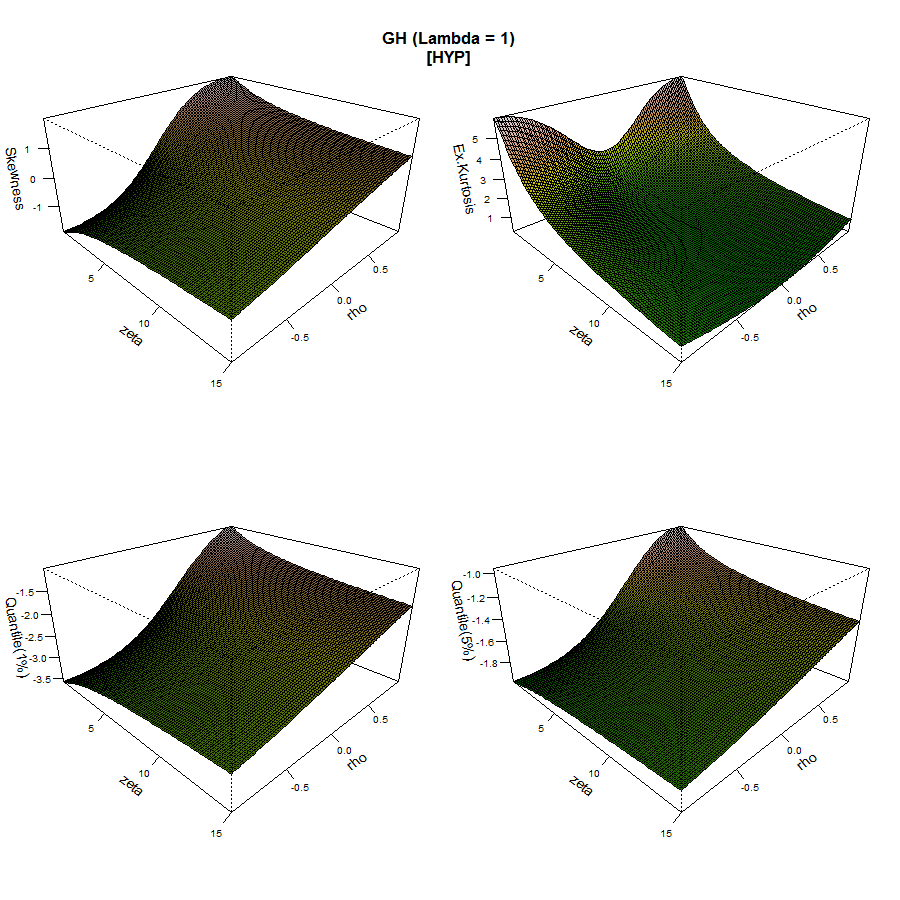
\includegraphics[scale=0.4, angle=0]{ghyp2.png}}
\subfloat[$\lambda=-0.5$(NIG)]{\label{fig:ghyp3}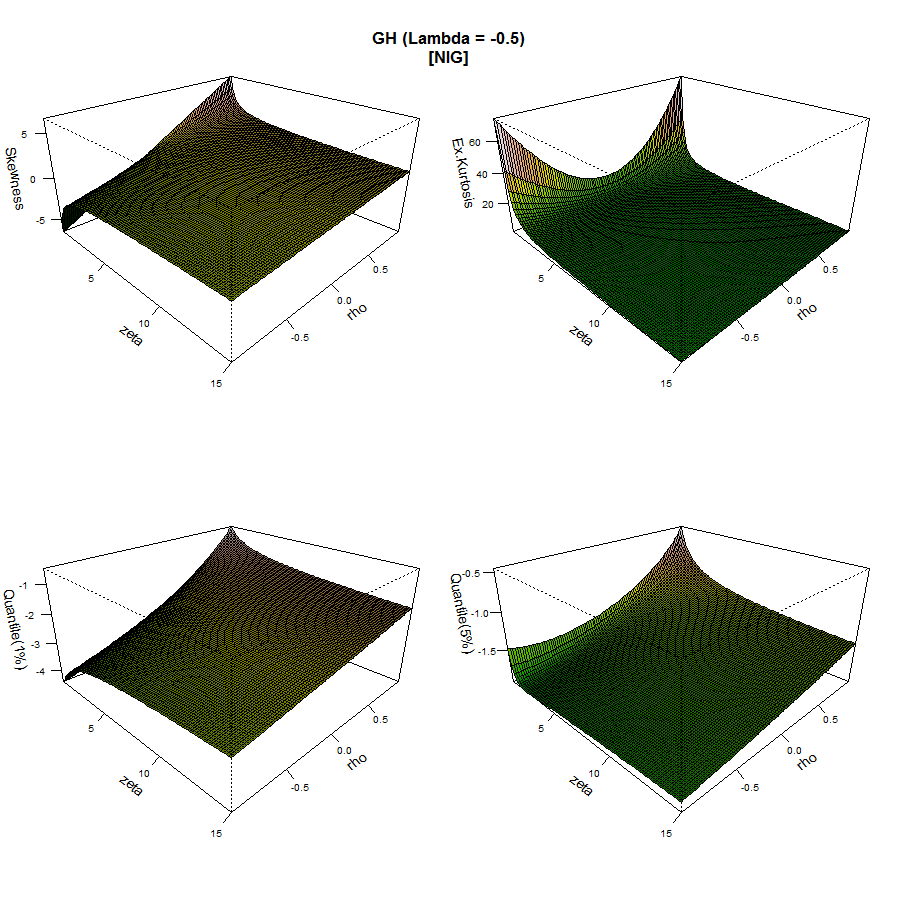
\includegraphics[scale=0.4, angle=0]{ghyp3.png}}
\caption[GH Distribution Skewness, Kurtosis and Quantile Surfaces]{GH Distribution Skewness, Kurtosis and Quantile Surfaces}\label{fig:ghsurface}
\end{figure}
\end{landscape}

\subsubsection{Johnson's Reparametrized SU Distribution}\label{jsu}
The reparametrized Johnson SU distribution, discussed in \citet{Rigby1}, is a
four parameter distribution denoted by $JSU\left(\mu,\sigma,\nu,\tau\right)$,
with mean $\mu$ and standard deviation $\sigma$ for all values of the skew and
shape parameters $\nu$ and $\tau$ respectively. The implementation is taken
from the GAMLSS package of \citet{Rigby1} and the reader is referred there for
further details.

\section{Fitting}\label{section:fitting}
Once a \verb@uGARCHspec@ has been defined, the \verb@ugarchfit@ method takes
the following arguments:
\begin{Schunk}
\begin{Sinput}
> args(ugarchfit)
\end{Sinput}
\begin{Soutput}
function (spec, data, out.sample = 0, solver = "solnp", solver.control = list(),
    fit.control = list(stationarity = 1, fixed.se = 0, scale = 0),
    ...)
NULL
\end{Soutput}
\end{Schunk}
The out.sample option controls how many data points from the end to keep for out
of sample forecasting, while the solver.control and fit.control provide additional
options to the fitting routine. Currently, 4 solvers are supported, with the main
one being the augmented Lagrange solver solnp of \citet{Ye} implemented in R by
\citet{Ghalanos1}. The main functionality, namely the GARCH dynamics and
conditional likelihood calculations are done in C for speed. For reference, there
is a benchmark routine called \verb@ugarchbench@ which provides a comparison of
rugarch against 2 published GARCH models with analytic standard errors, and a
small scale comparison with a commercial GARCH implementation.
The fitted object is of class \verb@uGARCHfit@ which can be passed to a variety
of other methods such as show (summary), plot, ugarchsim, ugarchforecast etc.
The following example illustrates its use, but the interested reader should
consult the documentation on the methods available for the returned class.
\begin{Schunk}
\begin{Sinput}
> spec = ugarchspec()
> data(sp500ret)
> fit = ugarchfit(spec = spec, data = sp500ret, solver.control = list(trace = 0))
> show(fit)
\end{Sinput}
\begin{Soutput}
*---------------------------------*
*          GARCH Model Fit        *
*---------------------------------*

Conditional Variance Dynamics
-----------------------------------
GARCH Model     : sGARCH(1,1)
Mean Model      : ARFIMA(1,0,1)
Distribution    : norm

Optimal Parameters
------------------------------------
        Estimate  Std. Error  t value Pr(>|t|)
mu      0.000517    0.000090   5.7620        0
ar1     0.834804    0.058900  14.1732        0
ma1    -0.865358    0.054076 -16.0028        0
omega   0.000001    0.000000   5.2865        0
alpha1  0.087730    0.007667  11.4428        0
beta1   0.904987    0.008387 107.9058        0

Robust Standard Errors:
        Estimate  Std. Error  t value Pr(>|t|)
mu      0.000517    0.000101   5.1181 0.000000
ar1     0.834804    0.048413  17.2435 0.000000
ma1    -0.865358    0.044909 -19.2691 0.000000
omega   0.000001    0.000001   2.1924 0.028351
alpha1  0.087730    0.029486   2.9753 0.002927
beta1   0.904987    0.028773  31.4530 0.000000

LogLikelihood : 17901.99

Information Criteria
------------------------------------

Akaike       -6.4805
Bayes        -6.4733
Shibata      -6.4805
Hannan-Quinn -6.4780

Q-Statistics on Standardized Residuals
------------------------------------
      statistic  p-value
Lag10     14.11 0.078859
Lag15     27.78 0.009717
Lag20     31.01 0.028675

H0 : No serial correlation

Q-Statistics on Standardized Squared Residuals
------------------------------------
      statistic p-value
Lag10     3.069  0.9299
Lag15     5.905  0.9495
Lag20     8.424  0.9716

ARCH LM Tests
------------------------------------
             Statistic DoF P-Value
ARCH Lag[2]      1.482   2  0.4765
ARCH Lag[5]      1.738   5  0.8841
ARCH Lag[10]     3.018  10  0.9810

Nyblom stability test
------------------------------------
Joint Statistic:  175.774
Individual Statistics:
mu      0.1978
ar1     0.2202
ma1     0.1678
omega  21.5725
alpha1  0.1341
beta1   0.1122

Asymptotic Critical Values (10% 5% 1%)
Joint Statistic:         1.49 1.68 2.12
Individual Statistic:    0.35 0.47 0.75

Sign Bias Test
------------------------------------
                   t-value      prob sig
Sign Bias           0.3309 7.407e-01
Negative Sign Bias  3.0036 2.680e-03 ***
Positive Sign Bias  2.4489 1.436e-02  **
Joint Effect       29.0989 2.135e-06 ***


Adjusted Pearson Goodness-of-Fit Test:
------------------------------------
  group statistic p-value(g-1)
1    20     182.8    8.624e-29
2    30     188.2    3.007e-25
3    40     230.3    5.779e-29
4    50     234.0    6.090e-26


Elapsed time : 1.628
\end{Soutput}
\end{Schunk}

\subsection{Fit Diagnostics}\label{section:diagnostics}
The summary method for the \verb@uGARCHfit@ object provides the parameters and
their standard errors (and a robust version), together with a variety of tests
which can also be called individually.

The \verb@inforcriteria@ method on a fitted or filtered object returns the
Akaike (AIC), Bayesian (BIC), Hannan-Quinn (HQIC) and Shibata (SIC) information
criteria to enable model selection by penalizing overfitting at different rates.
Formally, they may be defined as:
\begin{equation}\label{inforcriteria}
\begin{gathered}
  AIC = \frac{{ - 2LL}}
{N} + \frac{{2m}}
{N} \hfill \\
  BIC = \frac{{ - 2LL}}
{N} + \frac{{m{{\log }_e}\left( N \right)}}
{N} \hfill \\
  HQIC = \frac{{ - 2LL}}
{N} + \frac{{\left( {2m{{\log }_e}\left( {{{\log }_e}\left( N \right)} \right)} \right)}}
{N} \hfill \\
  SIC = \frac{{ - 2LL}}
{N} + {\log _e}\left( {\frac{{\left( {N + 2m} \right)}}
{N}} \right) \hfill \\
\end{gathered}
\end{equation}

The Q-Statistics are the test statistics from the Box-Pierce test on the
Standardized Residuals with $(10,15,20)$ lags and d.o.f the number of the
AR and MA parameters, and Squared Standardized Residuals with
$(10,15,20)$ lags and d.o.f the number of ARCH and GARCH parameters $(q,p)$
Looking at the summary report, the high p-values for the Standardized Squared
Residuals indicates that there is little chance of serial correlation at the
lags tested. The evidence for the Standardized Residuals is not as convincing
but one should consider other factors, particularly when it comes to forecasting
models.

The ARCH LM test of \citet{Engle1} tests the presence of ARCH effects by regressing
the squared residuals of a series against its own lags. Since the NULL is of No
ARCH effects, a high p-value, as evidenced by the summary indicates that the
GARCH model used was adequate to remove any such effects present prior to
fitting (i.e. it is a good idea to test the series prior to fitting a GARCH model!).

The \verb@signbias@ calculates the Sign Bias Test of \citet{EngleNg}, and is also
displayed in the summary. This tests the presence of leverage effects in the
standardized residuals (to capture possible misspecification of the GARCH model),
by regressing the squared standardized residuals on lagged negative and positive
shocks as follows:
\begin{equation}\label{signbias}
\hat z_t^2 = {c_0} + {c_1}{I_{{{\hat z}_{t - 1}} < 0}} + {c_2}{I_{{{\hat z}_{t - 1}} < 0}}{\hat z_{t - 1}} + {c_3}{I_{{{\hat z}_{t - 1}} \geqslant 0}}{\hat z_{t - 1}} + {u_t}
\end{equation}
where $I$ is the indicator function and $\hat z_t$ the estimated standardized residuals
from the GARCH process. The Null Hypotheses are $H_0:c_i=0$ (for $i=1,2,3$), and that
jointly $H_0:c_1=c_2=c_3=0$. As can be inferred from the summary of the previous
fit, there is significant Negative and Positive reaction to shocks. Using
instead a model such as the apARCH would likely alleviate these effects.

The \verb@gof@ calculates the chi-squared goodness of fit test, which compares
the empirical distribution of the standardized residuals with the theoretical
ones from the chosen density. The implementation is based on the test of
\citet{Palm1} which adjusts the tests in the presence on non-i.i.d. observations
by reclassifying the standardized residuals not according to their value (as in
the standard test), but instead on their magnitude, calculating the probability
of observing a value smaller than the standardized residual, which should be
identically standard uniform distributed. The function must take 2 arguments, the
fitted object as well as the number of bins to classify the values. In the
summary to the fit, a choice of $(20,30,40,50)$ bins is used, and from the
summary of the previous example it is clear that the Normal distribution does
not adequately capture the empirical distribution based on this test.

The \verb@nymblom@ test calculates the parameter stability test of \citet{Nyblom},
as well as the joint test. Critical values against which to compare the results
are displayed.

Finally, some informative plots can be drawn either interactively(which = 'ask'),
individually (which = 1:12) else all at once (which = 'all') as in Figure
\ref{fig:fitplot}.

\begin{landscape}
\begin{figure}[!ht]
\centering
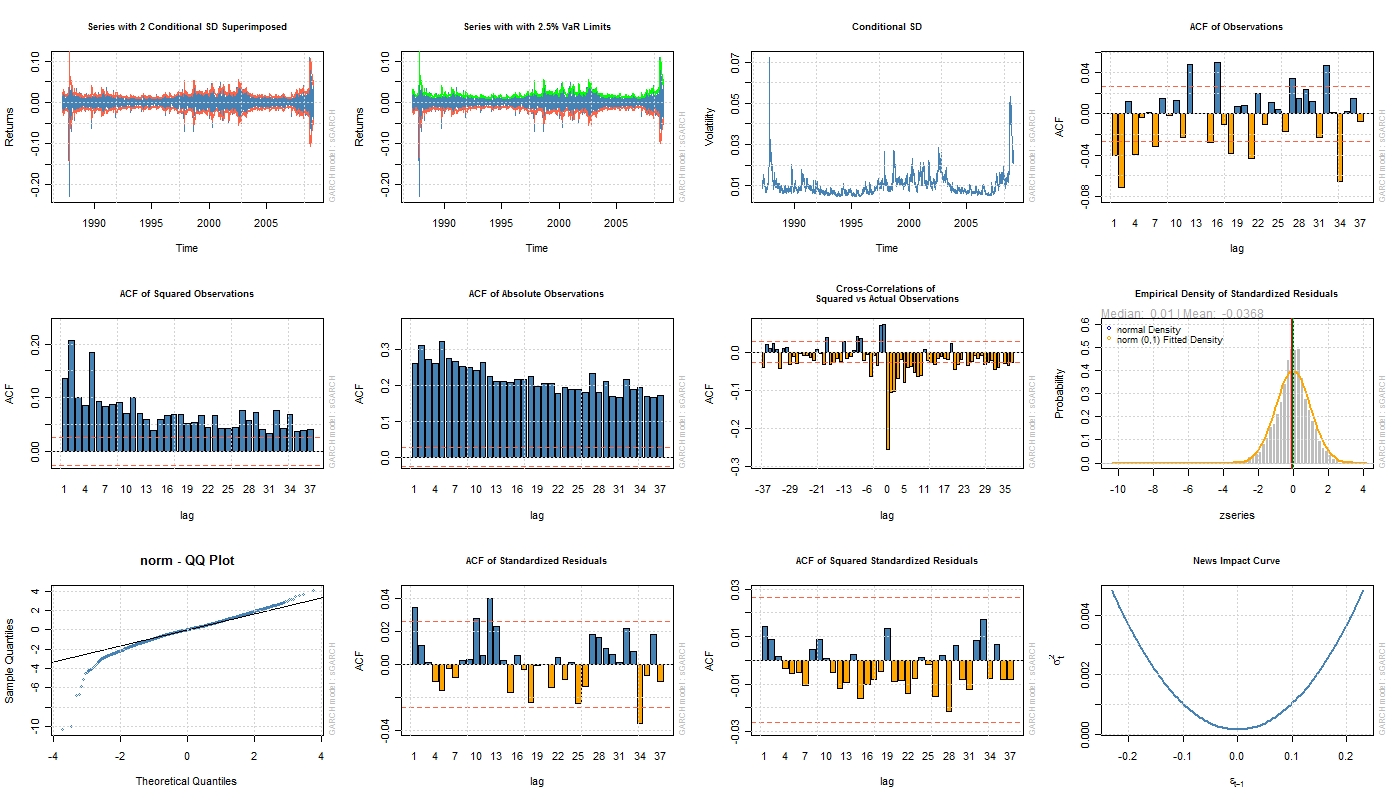
\includegraphics[width=22cm]{fitplot.png}
\caption[uGARCHfit Plots]{uGARCHfit Plots}\label{fig:fitplot}
\end{figure}
\end{landscape}

\section{Filtering}\label{section:filtering}
Sometimes it is desirable to simply filter a set of data with a predefined set
of parameters. This may for example be the case when new data has arrived and
one might not wish to re-fit. The \verb@ugarchfilter@ method does exactly that,
taking a \verb@uGARCHspec@ object with fixed parameters. Setting fixed or
starting parameters on the GARCH spec object may be done either through the
\verb@ugarchspec@ function when it is called (via the fixed.pars and start.pars
arguments to the function), else by using the \verb@setfixed<-@ and \verb@setstart<-@
method on the spec object. The example which follows explains how:
\begin{Schunk}
\begin{Sinput}
> data(sp500ret)
> spec = ugarchspec(variance.model = list(model = "apARCH"), distribution.model = "std")
> setfixed(spec) <- list(mu = 0.01, ma1 = 0.2, ar1 = 0.5, omega = 1e-05,
+     alpha1 = 0.03, beta1 = 0.9, gamma1 = 0.01, delta = 1, shape = 5)
> filt = ugarchfilter(spec = spec, data = sp500ret)
> show(filt)
\end{Sinput}
\begin{Soutput}
*------------------------------------*
*          GARCH Model Filter        *
*------------------------------------*

Conditional Variance Dynamics
--------------------------------------
GARCH Model     : apARCH(1,1)
Mean Model      : ARFIMA(1,0,1)
Distribution    : std

Filter Parameters
---------------------------------------

mu     1e-02
ar1    5e-01
ma1    2e-01
omega  1e-05
alpha1 3e-02
beta1  9e-01
gamma1 1e-02
delta  1e+00
shape  5e+00

LogLikelihood : 5627.291

Information Criteria
---------------------------------------

Akaike       -2.0345
Bayes        -2.0237
Shibata      -2.0345
Hannan-Quinn -2.0307

Q-Statistics on Standardized Residuals
---------------------------------------
      statistic p-value
Lag10      1231       0
Lag15      1240       0
Lag20      1248       0

H0 : No serial correlation

Q-Statistics on Standardized Squared Residuals
---------------------------------------
      statistic p-value
Lag10     179.2       0
Lag15     185.3       0
Lag20     189.8       0

ARCH LM Tests
---------------------------------------
             Statistic DoF P-Value
ARCH Lag[2]      171.5   2       0
ARCH Lag[5]      176.4   5       0
ARCH Lag[10]     177.9  10       0


Sign Bias Test
---------------------------------------
                   t-value      prob sig
Sign Bias            8.299 1.303e-16 ***
Negative Sign Bias   5.695 1.297e-08 ***
Positive Sign Bias   0.572 5.673e-01
Joint Effect        95.584 1.383e-20 ***


Adjusted Pearson Goodness-of-Fit Test:
---------------------------------------
  group statistic p-value(g-1)
1    20     27973            0
2    30     39420            0
3    40     49738            0
4    50     58614            0
\end{Soutput}
\end{Schunk}
The returned object is of class \verb@uGARCHfilter@ and shares many of the methods
as the \verb@uGARCHfit@ class. Additional arguments to the function are explained
in the documentation.

\section{Forecasting and the GARCH Bootstrap}\label{section:forecasting}
There are 2 types of forecasts available with the package. A rolling method,
whereby consecutive 1-ahead forecasts are created based on the out.sample option
set in the fitting routine, and an unconditional method for n>1 ahead forecasts.
It is also possible to combine the 2 creating a rather complicated object.
Additionally, it is possible to estimate the forecast density by means of the
\verb@ugarchboot@ method which implements the strategy described in
\citet{Pascual2}. This method also includes the option to include parameter
uncertainty via a monte carlo method. An example illustrates together with
Figure \ref{fig:bootplot} created using the plot command on the resulting
\verb@uGARCHboot@ object:
\begin{Schunk}
\begin{Sinput}
> data(sp500ret)
> spec = ugarchspec(variance.model = list(model = "eGARCH", garchOrder = c(1,
+     1)), mean.model = list(armaOrder = c(1, 1), arfima = FALSE),
+     distribution.model = "std")
> fit = ugarchfit(spec = spec, data = sp500ret, out.sample = 0,
+     solver = "solnp", solver.control = list(trace = 0))
> bootpred = ugarchboot(fit, method = "Partial", n.ahead = 120,
+     n.bootpred = 2000)
> show(bootpred)
\end{Sinput}
\begin{Soutput}
*-----------------------------------*
*     GARCH Bootstrap Forecast      *
*-----------------------------------*
Model : eGARCH
n.ahead : 120
Bootstrap method:  partial

Series (summary):
          min      q.25      mean     q.75      max forecast
t+1  -0.16970 -0.012573  0.000160 0.014647 0.087117 0.001266
t+2  -0.14045 -0.012198  0.000820 0.015917 0.088455 0.001043
t+3  -0.15926 -0.013462  0.000291 0.014136 0.097728 0.000880
t+4  -0.11009 -0.012629  0.000991 0.014653 0.088158 0.000761
t+5  -0.26634 -0.013391 -0.000698 0.013250 0.123779 0.000674
t+6  -0.24480 -0.012854 -0.000012 0.013587 0.089862 0.000610
t+7  -0.13669 -0.011373  0.001100 0.015331 0.097236 0.000564
t+8  -0.38366 -0.013117 -0.000036 0.014572 0.084560 0.000530
t+9  -0.26574 -0.012405  0.000074 0.014094 0.088518 0.000505
t+10 -0.21571 -0.011858  0.000652 0.013448 0.127877 0.000486
.....................

Sigma (summary):
          min    q0.25     mean    q0.75      max forecast
t+1  0.024673 0.024673 0.024673 0.024673 0.024673 0.024673
t+2  0.023374 0.023534 0.024438 0.024645 0.044920 0.024368
t+3  0.022176 0.022738 0.024186 0.025007 0.049329 0.024071
t+4  0.021142 0.022094 0.023938 0.025026 0.047645 0.023781
t+5  0.020084 0.021567 0.023656 0.024912 0.051322 0.023498
t+6  0.019257 0.021188 0.023476 0.024977 0.065176 0.023221
t+7  0.018390 0.020751 0.023252 0.024853 0.065914 0.022951
t+8  0.017720 0.020401 0.023005 0.024788 0.062841 0.022688
t+9  0.016862 0.020194 0.022880 0.024554 0.093453 0.022430
t+10 0.016061 0.019880 0.022697 0.024362 0.088260 0.022178
.....................
\end{Soutput}
\end{Schunk}
\begin{figure}
\centering
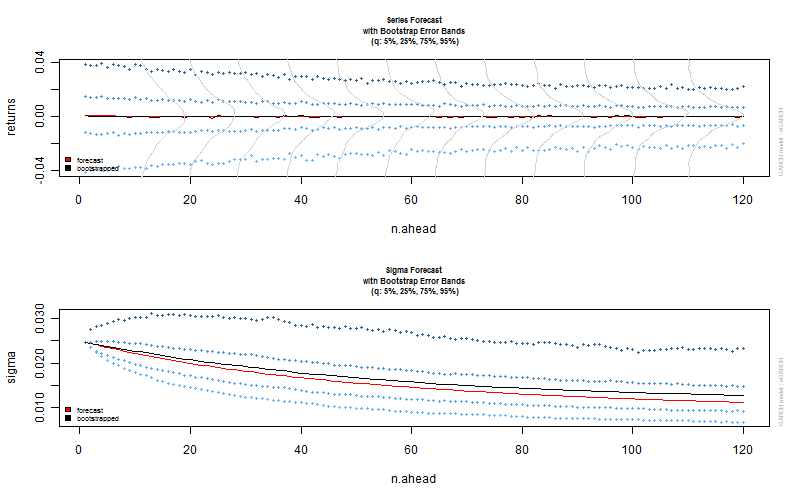
\includegraphics{boot.png}
\caption[GARCH Bootstrap Forecast Plots]{GARCH Bootstrap Forecast Plots}\label{fig:bootplot}
\end{figure}

\section{Simulation}\label{section:simulation}
Simulation may be carried out either directly on a fitted object (\verb@ugarchsim@)
else on a GARCH spec with fixed parameters (\verb@ugarchpath@). The \verb@ugarchsim@
method takes the following arguments:
\begin{Schunk}
\begin{Sinput}
> args(ugarchsim)
\end{Sinput}
\begin{Soutput}
function (fit, n.sim = 1000, n.start = 0, m.sim = 1, startMethod = c("unconditional",
    "sample"), presigma = NA, prereturns = NA, preresiduals = NA,
    rseed = NA, custom.dist = list(name = NA, distfit = NA),
    mexsimdata = NULL, vexsimdata = NULL, ...)
NULL
\end{Soutput}
\end{Schunk}
where the n.sim indicates the length of the simulation while m.sim the number of
independent simulations. For reasons of speed, when n.sim is large relative to
m.sim, the simulation code is executed in C, while for large m.sim a special
purpose C++ code (using Rcpp and RcppArmadillo) is used which was found to lead
to significant speed increase. Key to replicating results is the rseed argument
which is used to pass a user seed to initialize the random number generator, else
one will be assigned by the program. In any case, the returned object, of class
\verb@uGARCHsim@ (or \verb@uGARCHpath@) contains a slot with the seed(s) used.
\section{Rolling Estimation}\label{section:rolling}
The \verb@ugarchroll@ method allows to perform a rolling estimation and
forecasting of a model/dataset combination, optionally returning the VaR at
specified levels. More importantly, it returns the distributional forecast
parameters necessary to calculate any required measure on the forecasted density.
The following example illustrates the use of the method where use is also made
of the parallel option and run on 10 cores. Figure \ref{fig:roll} is generated
by calling the plot function on the returned \verb@uGARCHroll@ object.
Additional methods, and more importantly extractor functions can be found in the
documentation.
\begin{Schunk}
\begin{Sinput}
> data(sp500ret)
> spec = ugarchspec(variance.model = list(model = "eGARCH"), distribution.model = "jsu")
> roll = ugarchroll(spec, data = sp500ret, n.ahead = 1, forecast.length = 500,
+     refit.every = 25, refit.window = "recursive", parallel = TRUE,
+     parallel.control = list(pkg = "snowfall", cores = 10), solver = "solnp",
+     solver.control = list(tol = 1e-05, delta = 1e-06, trace = 0),
+     calculate.VaR = TRUE, VaR.alpha = c(0.01, 0.05))
\end{Sinput}
\begin{Sinput}
> report(roll, type = "VaR", n.ahead = 1, VaR.alpha = 0.01, conf.level = 0.95)
\end{Sinput}
\begin{Soutput}
VaR Backtest Report
===========================================
Model:                  eGARCH-jsu
Backtest Length:        500
Data:                   SP500RET

==========================================
alpha:                  1%
Expected Exceed:        5
Actual VaR Exceed:      9
Actual %:               1.8%

Unconditional Coverage (Kupiec)
Null-Hypothesis:        Correct Exceedances
LR.uc Statistic:        2.613
LR.uc Critical:         3.841
LR.uc p-value:          0.106
Reject Null:            NO

Conditional Coverage (Christoffersen)
Null-Hypothesis:        Correct Exceedances &
                        Independence of Failures
LR.cc Statistic:        2.943
LR.cc Critical:         5.991
LR.cc p-value:          0.23
Reject Null:            NO
\end{Soutput}
\begin{Sinput}
> report(roll, type = "fpm")
\end{Sinput}
\begin{Soutput}
GARCH Roll Mean Forecast Performance Measures
---------------------------------------------
Model : eGARCH
no.refits : 20
n.ahead   : 1
n.rolls   : 500

    n.ahead.1
MSE 4.080e-04
MAE 1.295e-02
DAC 5.500e-01
N   5.000e+02
\end{Soutput}
\end{Schunk}
\begin{figure}
\centering
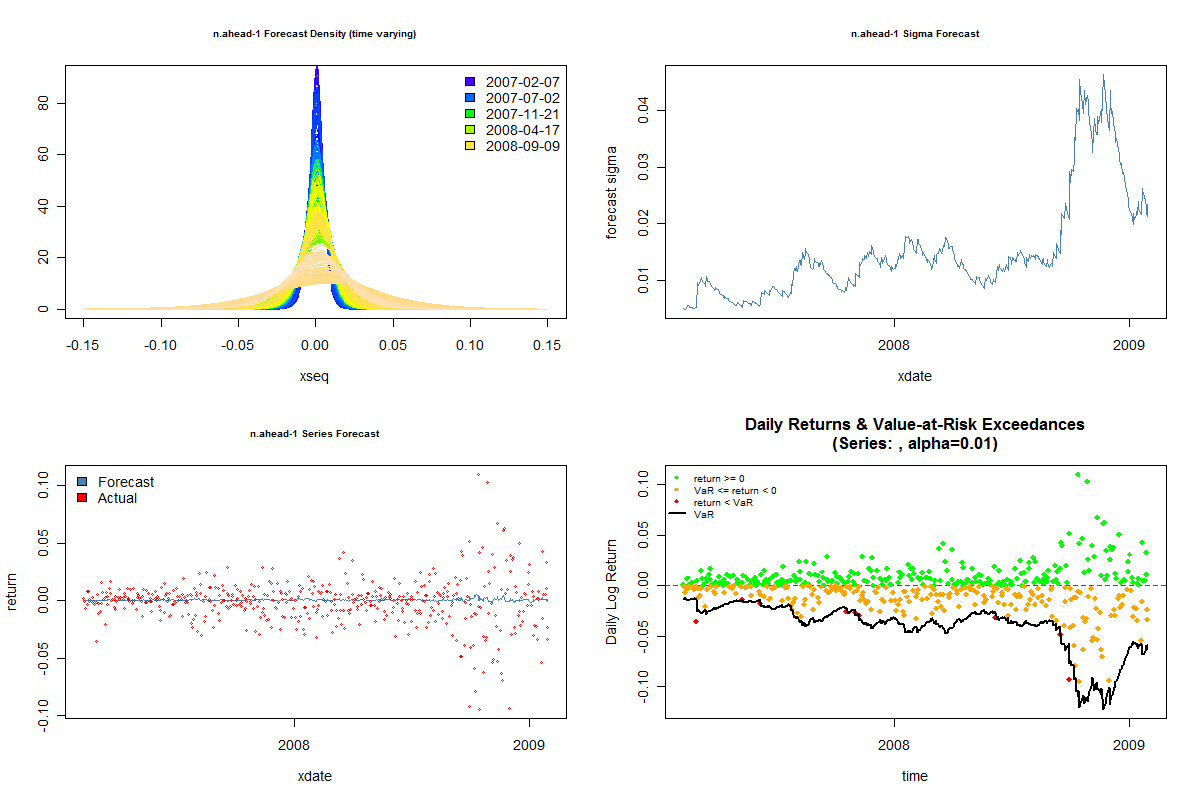
\includegraphics{roll.png}
\caption[GARCH Rolling Forecast Plots]{GARCH Rolling Forecast Plots}\label{fig:roll}
\end{figure}

\section{Simulated Parameter Distribution and RMSE}\label{section:ugarchdist}
It is sometimes instructive to be able to investigate the underlying
density of the estimated parameters under different models. The \verb@ugarchdistribution@
method performs a monte carlo experiment by simulating and fitting a model
multiple times and for different 'window' sizes. This allows to obtain some insight
on the consistency of the parameter estimates as the data window increases by
looking at the rate of decrease of the Root Mean Squared Error and whether we
have $\sqrt N$ consistency. This is a computationally expensive exercise and as
such should only be undertaken in the presence of ample computing power and RAM.
As in other functions, parallel functionality is enabled if available.
The example which follows illustrates an instance of this test on one model and
one set of parameters. Figures \ref{fig:dist1} and \ref{fig:dist2} complete this
example.
\begin{Schunk}
\begin{Sinput}
> spec = ugarchspec(variance.model = list(model = "gjrGARCH"),
+     distribution.model = "ged")
> print(persistence(pars = unlist(list(mu = 0.001, ar1 = 0.4, ma1 = -0.1,
+     omega = 1e-06, alpha1 = 0.05, beta1 = 0.9, gamma1 = 0.05,
+     shape = 1.5)), distribution = "ged", model = "gjrGARCH"))
\end{Sinput}
\begin{Soutput}
persistence
      0.975
\end{Soutput}
\begin{Sinput}
> setfixed(spec) <- list(mu = 0.001, ar1 = 0.4, ma1 = -0.1, omega = 1e-06,
+     alpha1 = 0.05, beta1 = 0.9, gamma1 = 0.05, shape = 1.5)
> dist = ugarchdistribution(fitORspec = spec, n.sim = 2000, n.start = 1,
+     m.sim = 100, recursive = TRUE, recursive.length = 6000, recursive.window = 1000,
+     rseed = 1066, solver = "solnp", solver.control = list(trace = 0),
+     parallel = TRUE, parallel.control = list(pkg = "snowfall",
+         cores = 20))
> show(dist)
\end{Sinput}
\begin{Soutput}
*------------------------------------*
*    GARCH Parameter Distribution    *
*------------------------------------*
Model : gjrGARCH
No. Paths (m.sim) : 100
Length of Paths (n.sim) : 2000
Recursive : TRUE
Recursive Length : 6000
Recursive Window : 1000

Coefficients: True vs Simulation Mean (Window-n)
                    mu     ar1       ma1      omega   alpha1   beta1   gamma1
true-coef   0.00100000 0.40000 -0.100000 1.0000e-06 0.050000 0.90000 0.050000
window-2000 0.00097122 0.39691 -0.097773 1.0672e-06 0.046603 0.90054 0.051852
window-3000 0.00101426 0.38922 -0.089512 1.0209e-06 0.047097 0.90072 0.052936
window-4000 0.00099796 0.39372 -0.095054 1.0219e-06 0.049798 0.90056 0.047732
window-5000 0.00099337 0.40143 -0.102950 1.0081e-06 0.048943 0.90087 0.049678
window-6000 0.00098468 0.39561 -0.096174 1.0102e-06 0.049052 0.90009 0.050879
             shape
true-coef   1.5000
window-2000 1.4944
window-3000 1.4960
window-4000 1.4929
window-5000 1.4899
window-6000 1.4902
\end{Soutput}
\end{Schunk}

\begin{landscape}
\begin{figure}[!ht]
\centering
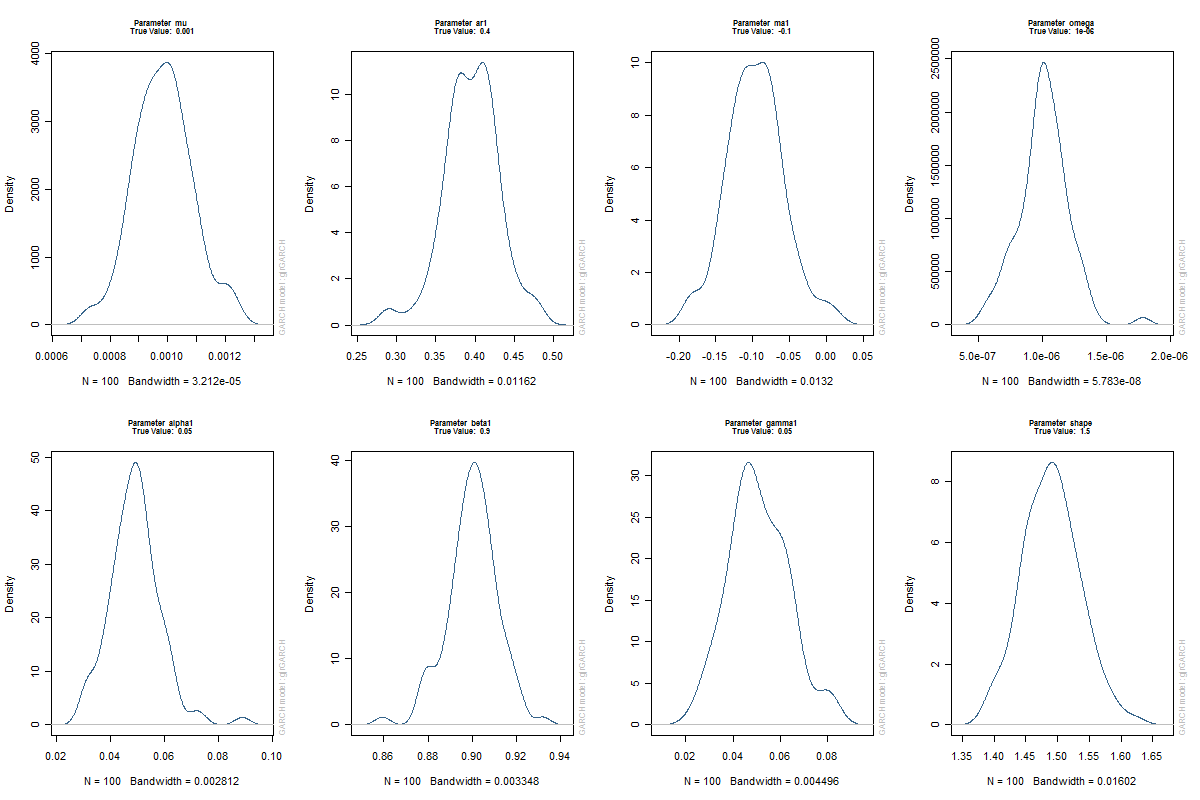
\includegraphics[width=22cm]{dist1.png}
\caption[GARCH Simulated Parameters Density]{Simulated Parameter Density}\label{fig:dist1}
\end{figure}
\begin{figure}[!ht]
\centering
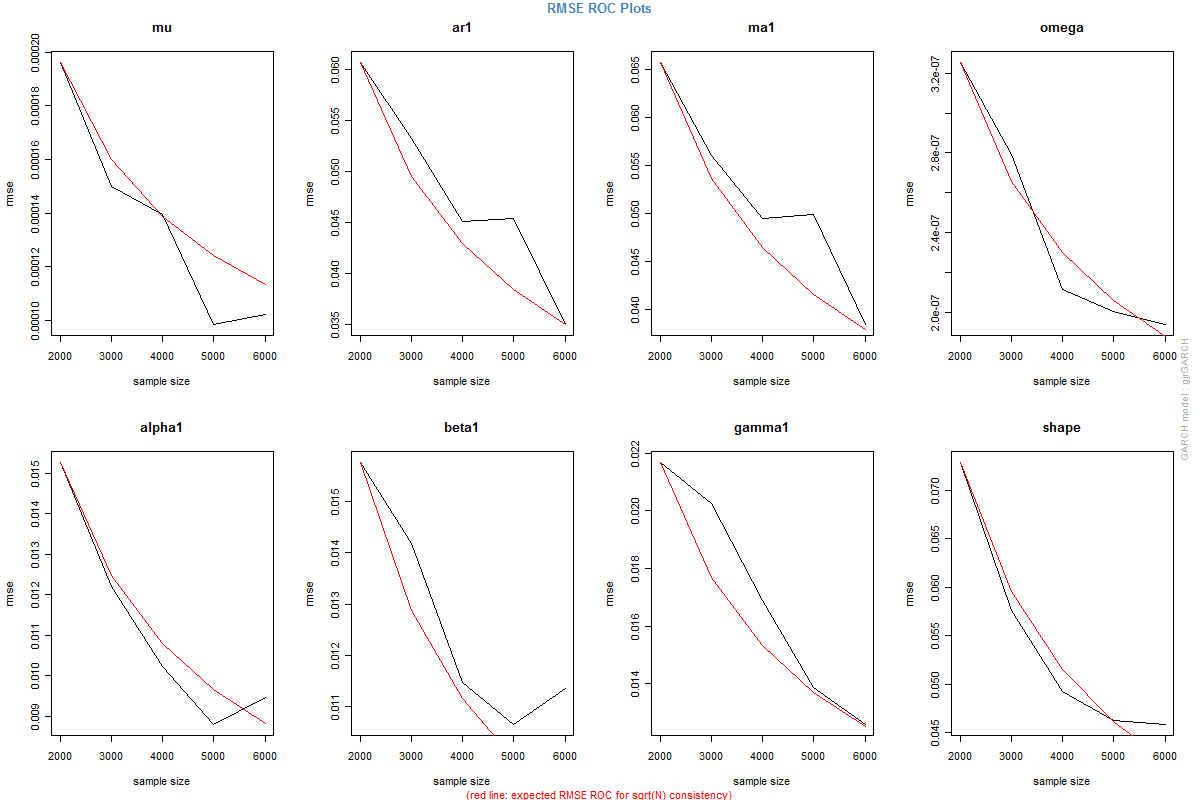
\includegraphics[width=22cm]{dist11.png}
\caption[GARCH Parameters RMSE Rate of Change]{RMSE Rate of Change}\label{fig:dist2}
\end{figure}
\begin{figure}[!ht]
\centering
\subfloat[Bivariate Parameter Plots]{\label{fig:dist3}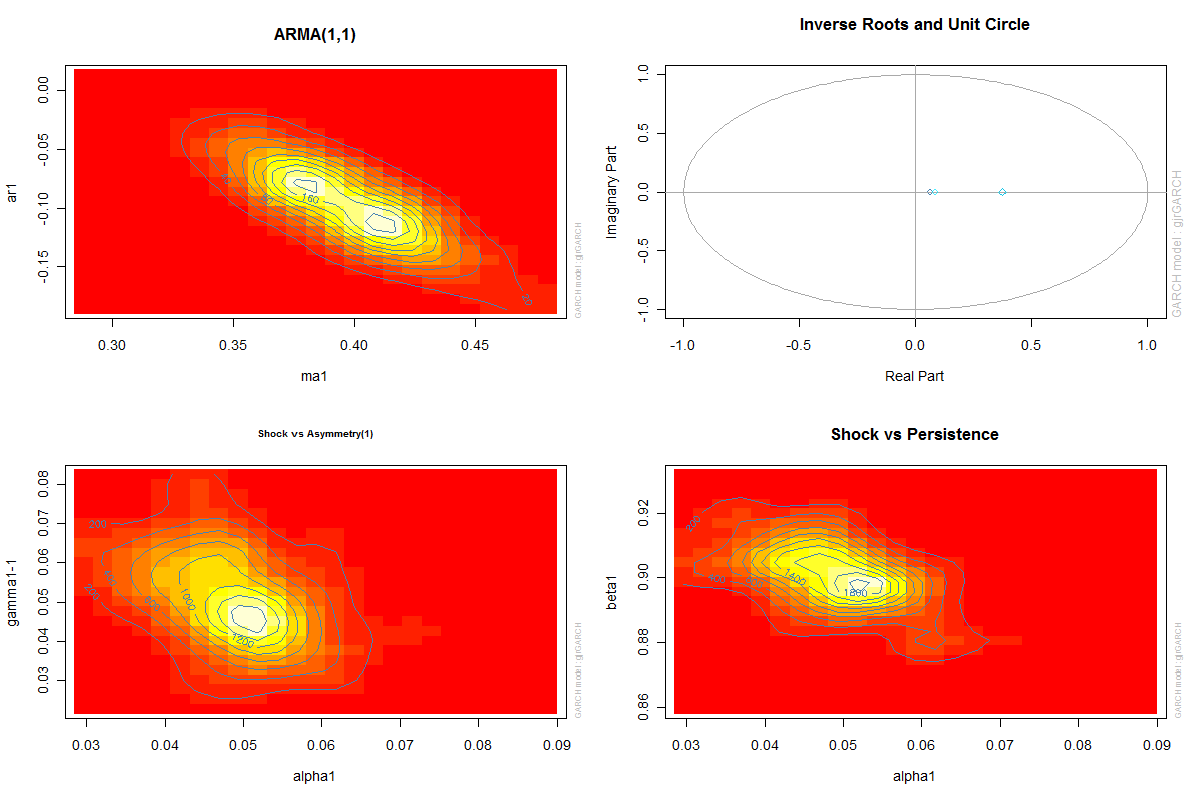
\includegraphics[scale=0.4, angle=0]{dist2.png}}
\subfloat[GARCH Stat Plots]{\label{fig:dist4}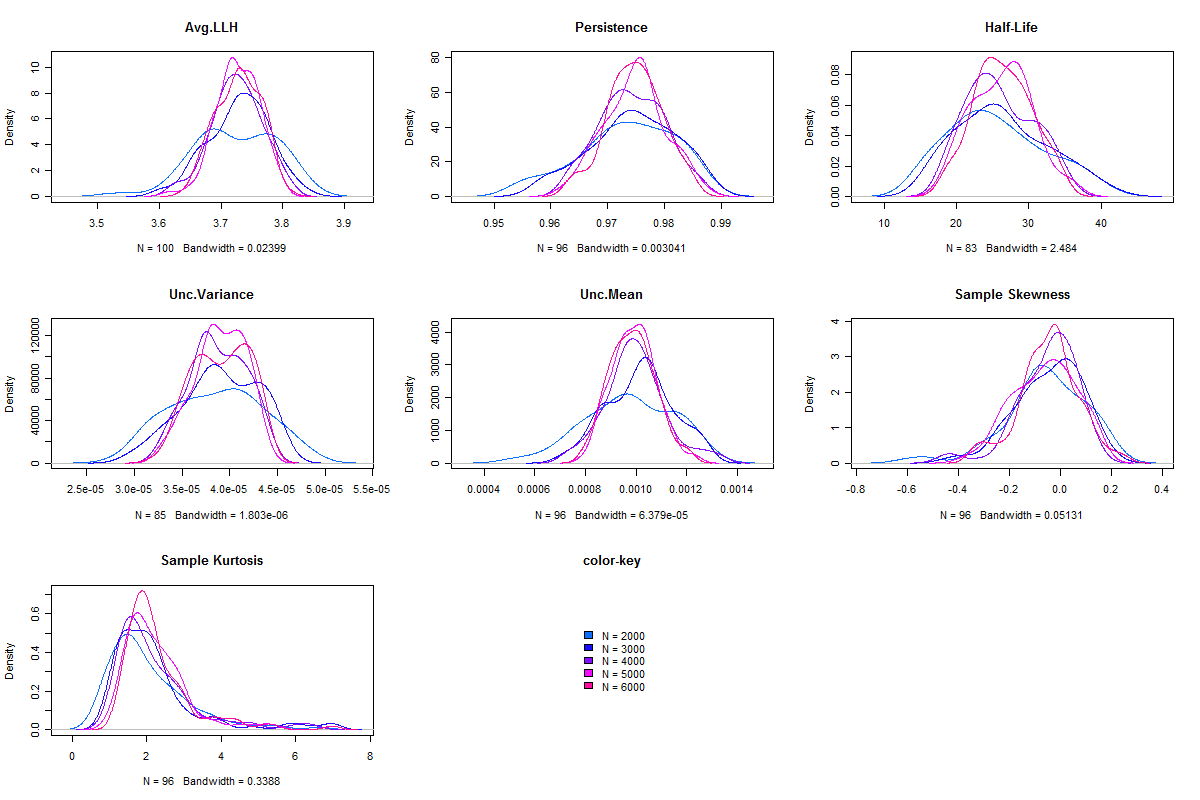
\includegraphics[scale=0.4, angle=0]{dist3.png}}
\caption[GARCH Simulated Parameters Density]{GARCH Simulated Parameters Density}\label{fig:dist3}
\end{figure}
\end{landscape}

\section{The ARFIMAX Model with constant variance}\label{section:arfima}
The \verb@rugarch@ package implements an additional set of methods and classes,
mirroring those of the GARCH specification, for modelling ARFIMAX processes
with constant variance via Maximum Likelihood. With the exception of plots, the
functionality is very similar to that covered so far for GARCH methods. The main
functions are \verb@arfimaspec@, \verb@arfimafit@, \verb@arfimaforecast@,
\verb@arfimasim@, \verb@arfimapath@, \verb@arfimadistirbution@ and \verb@arfimaroll@.
The usual extractor, inference and summary methods are replicated for all the
ARFIMA classes and the user should consult the documentation for further details.

\section{Miscellaneous Functions}\label{section:misc}
There are a number of plain R functions exported in the package the most important
of which are the \verb@WeekDayDummy@ (creates a dummy, day of the week variable
given a set of dates), \verb@ForwardDates@ (to generate A POSIXct vector of future
dates), \verb@BerkowitzLR@ which implements the density forecast test of
\citet{Berkowitz}, and the \verb@DACTest@ function which implements the Directional
Accuracy tests of \citet{Anatolyev} and \citet{Pesaran}. The unconditional and
conditional VaR exceedances tests are currently not exported but may be called
via rugarch:::.VaRreport (and the associated plot via rugarch:::.VaRplot).

\section{FAQs and Guidelines}\label{section:faqs}
This section provides for answers to some Frequently Asked Questions (Q) as well
as Guidelines (G) for the use of the \verb@rugarch@ package.\\
\\
\textbf{Q: Does the package support parallel computation?}\\
\\
Yes. Most functions for which parallel functionality was deemed beneficial
include the additional options of 'parallel' and 'parallel.control'. For Unix
based systems the multicore package of \citet{Urbanek} provides
for a very efficient parallel apply on multiple cores. For Windows and all
systems, the snowfall package of \citet{Knaus} allows for socket based parallel
apply which does not include shared memory of objects and can therefore be very
expensive. This is definitely not as efficient as multicore, but the only option
currently on windows systems. Some extra thought is required when using the
snowfall parallel functionality as there is a trade-off to consider between the
number of cores committed via socket, the overhead for setting up each new
socket and the number of parallel iterations. As an example consider the
following:
\begin{Schunk}
\begin{Sinput}
> library(rugarch)
\end{Sinput}
\begin{Soutput}
rugarch (version 1.0) initialized.
\end{Soutput}
\begin{Sinput}
> data(dji30ret)
> spec = ugarchspec()
> mspec = multispec(replicate(spec, n = 30))
> print(system.time(multifit(multispec = mspec, data = dji30ret[,
+     1:30], parallel = TRUE, parallel.control = list(pkg = "snowfall",
+     cores = 20))))
\end{Sinput}
\begin{Soutput}
   user  system elapsed
   1.08    1.88   24.00
\end{Soutput}
\begin{Sinput}
> print(system.time(multifit(multispec = mspec, data = dji30ret[,
+     1:30], parallel = TRUE, parallel.control = list(pkg = "snowfall",
+     cores = 5))))
\end{Sinput}
\begin{Soutput}
   user  system elapsed
   0.34    0.23   15.78
\end{Soutput}
\begin{Sinput}
> print(system.time(multifit(multispec = mspec, data = dji30ret[,
+     1:30], solver.control = list(trace = 0), parallel = FALSE,
+     parallel.control = list(pkg = "snowfall", cores = 10))))
\end{Sinput}
\begin{Soutput}
   user  system elapsed
  49.15    0.00   49.15
\end{Soutput}
\end{Schunk}
It is clear that the overhead for using 20 cores is too high for the size of
this problem, whereas using 5 cores does lead to a doubling of performance
versus the non-parallel version. Also note that prior to using the snowfall
package, this should be manually loaded by the user, since strange behavior has
been observed when the package tries to load the snowfall itself.\\
\\
\textbf{Q: My model does not converge, what can I do?}\\
\\
There are several avenues to consider here. The package offers 4 different
solvers, namely 'solnp', 'gosolnp', 'nlminb' and 'L-BGFS-U' (from optim).
Each solver has its own merits, and control parameters which may, and should be
passed, via the solver.control list in the fitting routines, depending on your
particular data. For problems where neither 'solnp' nor 'nlminb' seem to work,
try the 'gosolnp' solver which does a search of the parameter space based on a
truncated normal distribution for the parameters and then initializes multiple
restarts of the 'solnp' solver based on the best identified candidates. The
numbers of randomly generated parameters (n.sim) and solver restarts (n.restarts)
can be passed via the solver.control list. Additionally, in the fit.control list
of the fitting routines, the option to perform scaling of the data prior to
fitting usually helps, although it is not available under some setups. Finally,
consider the amount of data you are using for modelling GARCH processes,
which leads to another FAQ below.\\
\\
\textbf{Q: How much data should I use to model GARCH processes with confidence?}\\
The distribution of the parameters varies by model, and is left to the reader to
consult relevant literature on this. However, using 100 data points to try and
fit a model is unlikely to be a sound approach as you are unlikely to get very
efficient parameter estimates. The \verb@rugarch@ package does provide a method
(\verb@ugarchdistribution@) for simulating from a pre-specified model, data of
different sizes, fitting the model to the data, and inferring the distribution
of the parameters as well as the RMSE rate of change as the data length
increases. This is a very computationally expensive way to examine the
distribution of the parameters (but the only way in the non-Bayesian world), and
as such should be used with care and in the presence of ample computing power.\\
\\
\textbf{Q: Where can one find more examples?}\\
\\
The package has a folder called 'rugarch.tests' which contains many tests
which I use for debugging and checking. The files in the folder should be
'sourced' by the user, and the 'runtests.R' file contains some wrapper functions
which describe what each test does, and optionally runs chosen tests. The
output will be a combination of text files (.txt) and figures (either .eps or
.png) in an output directory which the user can define in the arguments to the
wrapper function 'rugarch.runtests'. It is quite instructive to read and
understand what each test is doing prior to running it...\\

\begin{thebibliography}{}

\bibitem[Alexander (2001)]{ALEXANDER}
Alexander, C. (2001).
\newblock Orthogonal GARCH.
\newblock In \emph{Mastering risk, 2}, pp.~21--38.

\bibitem[Anatolyev and Gerko (2005)]{Anatolyev}
Anatolyev, S. and Gerko, A. (2005).
\newblock  A trading approach to testing for predictability.
\newblock In \emph{Journal of Business and Economic Statistics, 23(4)},
pp.~455--461.

\bibitem[de Athayde and Flores (2002)]{ATHAYDE}
de Athayde, G.M. and Flores Jr, R.G. (2002).
\newblock On Certain Geometric Aspects of Portfolio Optimisation with Higher Moments.
\newblock In \emph{mimeo}.

\bibitem[Berkowitz (2001)]{Berkowitz}
Berkowitz, J. (2001).
\newblock Testing density forecasts with applications to risk management.
\newblock In \emph{Journal of Business and Economic Statistics 19(4)}, pp.~465--474.

\bibitem[Blaesild (1981)]{BLAESILD}
Blaesild, P. (1981).
\newblock The two-dimensional hyperbolic distribution and related distributions, with an application to Johannsen's bean data.
\newblock In \emph{Biometrika, 68(1)}, pp.~251--263.

\bibitem[Bollerslev (1986)]{Bollerslev1}
Bollerslev, T. (1986).
\newblock Generalized autoregressive conditional heteroskedasticity.
\newblock In \emph{Journal of Econometrics, 31(3)}, pp.~307--327.

\bibitem[Bollerslev (1987)]{Bollerslev2}
Bollerslev, T. (1987).
\newblock A Conditionally Heteroskedastic Time Series Model for Speculative Prices and Rates of Return.
\newblock In \emph{Review of Economics and Statistics, 69}, pp.~542--547

\bibitem[Box and Cox (1964)]{Box1}
Box, G. and Cox, D.R. (1964).
\newblock An analysis of transformations.
\newblock In \emph{Journal of the Royal Statistical Society, Series B  (Methodological)}, pp.~211--252.

\bibitem[Box, Jenkins and Reinsel (1970)]{Box2}
Box, G. and Jenkins, G.M. and Reinsel, G.C.
\newblock Time Series Analysis: Forecasting and Control.
\newblock In \emph{Holden-Day}.

\bibitem[Broda and Paolella (2009)]{BRODA}
Broda, S.A. and Paolella, M.S. (2009).
\newblock CHICAGO: A Fast and Accurate Method for Portfolio Risk Calculation.
\newblock In \emph{Journal of Financial Econometrics, 7(14)}, pp.~412--436.

\bibitem[Chen et al. (2007)]{CHEN}
Chen, Y. and H{\"{a}}rdle, W. and Spokoiny, V. (2007).
\newblock Portfolio value at risk based on independent component analysis.
\newblock In \emph{Journal of Computational and Applied Mathematics, 205(1)}, pp.~594--607.

\bibitem[Ding, Granger and Engle (1993)]{Ding1}
Ding, Z. and Granger, C.W.J. and Engle, R.F. (1993).
\newblock A long memory property of stock market returns and a new model.
\newblock In \emph{Journal of Empirical Finance, 1(1)}, pp.~83--106.

\bibitem[Engle (1982)]{Engle1}
Engle, R.F. (1982).
\newblock Autoregressive conditional heteroscedasticity with estimates of the variance of United Kingdom inflation.
\newblock In \emph{Econometrica, 50(4)}, pp.~987--1007.


\bibitem[Engle and Bollerslev (1986)]{Engle2}
Engle, R.F. and Bollerslev, T. (1986).
\newblock Modeling the Persistence of Conditional Variances.
\newblock In \emph{Econometric Reviews, 5}, pp.~1--50.

\bibitem[Engle and Ng (1993)]{EngleNg}
Engle, R.F. and Ng, V.K. (1993).
\newblock Measuring and testing the impact of new on volatility.
\newblock In \emph{Journal of Finance, 48}, pp.~1749--1778.


\bibitem[Engle (1987)]{EngleLilienRobbins}
Engle, R.F. and Lilien, D.M. and Robbins, R.P. (1987)
\newblock Estimating Time Varying Risk Premia in the Term Structure: The ARCH-M Model.
\newblock In \emph{Econometrica, 55(2)}, pp.~391?--407.

\bibitem[Engle (1996)]{EngleMezrich}
Engle, R. and Mezrich, J. (1996)
\newblock GARCH for Groups.
\newblock In \emph{RISK, (9)}, pp.~36--40.

\bibitem[Fernandez and Steel (1998)]{Fernandez1}
Fernandez, C. and Steel, M.F. (1998).
\newblock On Bayesian Modeling of Fat Tails and Skewness.
\newblock In \emph{Journal of the American Statistical Association, 93(441)}, pp.~359--371.

\bibitem[Ferreira and Steel (2006)]{Ferreira1}
Ferreira, J.T. and Steel, M.F. (2006).
\newblock A constructive representation of univariate skewed distributions.
\newblock In \emph{Journal of the American Statistical Association, 101(474)}, pp.~823--829.

\bibitem[Ghalanos and Theussl (2011)]{Ghalanos1}
Ghalanos, A. and Theussl, S. (2011)
\newblock Rsolnp: General Non-linear Optimization Using Augmented Lagrange Multiplier Method.
\newblock In \emph{manual}.

\bibitem[Glosten, Jagannathan and Runkle (1993)]{Glosten1}
Glosten, L.R. and Jagannathan, R. and Runkle, D.E. (1993).
\newblock On the relation between the expected value and the volatility of the nominal excess return on stocks.
\newblock In \emph{Journal of Finance, 48(5)}, pp.~1779--1801.

\bibitem[Geweke (1986)]{Geweke}
Geweke, J. (1986).
\newblock Modeling the Persistence of Conditional Variances: A Comment.
\newblock In \emph{Econometric Reviews, (5)}, pp.~57--61.

\bibitem[Hansen (1990)]{HANSEN1}
Hansen, B.E. (1990).
\newblock Lagrange multiplier tests for parameter instability in non-linear models.
\newblock In \emph{mimeo}.

\bibitem[Hansen (1994)]{HANSEN2}
Hansen, B.E. (1994).
\newblock Autoregressive conditional density estimation.
\newblock In \emph{International Economic Review}, pp.~705--730.

\bibitem[Hentschel (1995)]{Hentschel1}
Hentschel, L. (1995).
\newblock All in the family Nesting symmetric and asymmetric GARCH models.
\newblock In \emph{Journal of Financial Economics, 39(1)}, pp.~71--104.

\bibitem[Higgins and Bera (1992)]{Higgins}
Higgins, M. L. and Bera, A. K. (1992).
\newblock A Class of Nonlinear ARCH Models.
\newblock In \emph{International Economic Review, 33}, pp.~137--158.

\bibitem[Knaus (2010)]{Knaus}
Knaus, J. (2010).
\newblock snowfall: Easier cluster computing (based on snow).
\newblock \emph{Manual}.

\bibitem[Mandelbrot (1963)]{Mandelbrot}
Mandelbrot, B. (1963).
\newblock The variation of certain speculative prices.
\newblock In \emph{Journal of business, 36(4)}, pp.394--419.

\bibitem[Nelson (1991)]{Nelson}
Nelson, D.B (1991).
\newblock Conditional Heteroskedasticity in Asset Returns: A New Approach.
\newblock In \emph{Econometrica, 59}, pp.347--370.

\bibitem[Nyblom (1989)]{Nyblom}
Nelson, D.B (1989).
\newblock Testing for the Constancy of Parameters Over Time.
\newblock In \emph{Journal of the American Statistical Association, 84(405)}, pp.223--230.

\bibitem[Palm and Vlaar (1997)]{Palm1}
Palm, F.C. and Vlaar, P.J.G. (1997).
\newblock Simple diagnostic procedures for modeling financial time series.
\newblock In \emph{Allgemeines statistisches Archiv: Organ der Deutschen Statistischen Gesellschaft, 81}, pp.~85--101.

\bibitem[Pantula (1986)]{Pantula}
Pantula, S. G. (1986).
\newblock Comment: Modelling the persistence of conditional variances.
\newblock In \emph{Econometric Reviews, (5)}, pp.~71--73.

\bibitem[Rigby (2005)]{Rigby1}
Rigby, R. A. and Stasinopoulos, D. M. (2005).
\newblock Generalized Additive Models for Location, Scale and Shape.
\newblock In \emph{Journal of the Royal Statistical Society. Series C (Applied Statistics), 54(3)}, pp.~507--554.

\bibitem[Pascual, Romo and Ruiz (2004)]{Pascual1}
Pascual, L. and Romo, J. and Ruiz, E. (2004).
\newblock Bootstrap predictive inference for ARIMA processes.
\newblock In \emph{Journal of Time Series Analysis, 25(4)}, pp.~449--465.

\bibitem[Pascual, Romo and Ruiz (2006)]{Pascual2}
Pascual, L. and Romo, J. and Ruiz, E. (2006).
\newblock Bootstrap prediction for returns and volatilities in GARCH models.
\newblock In \emph{Computational Statistics and Data Analysis, 50(9)}, pp.~2293--2312.

\bibitem[Pesaran and  Timmermann (1992)]{Pesaran}
Pesaran, M.H. and Timmermann, A. (1992).
\newblock A simple nonparametric test of predictive performance.
\newblock In \emph{Journal of Business and Economic Statistics, 10(4)}, pp.~461--465.

\bibitem[van der Weide (2002)]{WEIDE1}
van der Weide, R. (2002).
\newblock GO-GARCH: a multivariate generalized orthogonal GARCH model.
\newblock In \emph{Journal of Applied Econometrics, 17(5)}, pp.~549--564.

\bibitem[van der Weide (2004)]{WEIDE2}
van der Weide, R. (2004).
\newblock Wake me up before you GO-GARCH.
\newblock In \emph{Computing in Economics and Finance (2004)}.

\bibitem[van der Weide and Boswijk (2008)]{WEIDE3}
van der Weide, R. and Boswijk, P. (2008).
\newblock Method of moments estimation of GO-GARCH models.
\newblock In \emph{mimeo}.

\bibitem[Zhang and Chan (2009)]{ZHANG}
Zhang, K. and Chan, L. (2009).
\newblock Efficient factor GARCH models and factor-DCC models.
\newblock In \emph{Quantitative Finance, 9(1)}, pp.~71--91.

\bibitem[Schmidt et al. (2006)]{SCHMIDT}
Schmidt, R. and Hrycej, T. and St{\"{u}}tzle, E. (2006).
\newblock Multivariate distribution models with generalized hyperbolic margins.
\newblock In \emph{Computational statistics and data analysis, 50(8)}, pp.~2065--2096.

\bibitem[Schwert (1990)]{Schwert}
Schwert, W (1990).
\newblock Stock volatility and the crash of '87.
\newblock In \emph{Review of financial Studies (3)}, pp.~77--102.

\bibitem[Taylor (1986)]{Taylor}
Taylor, S. (1986).
\newblock Modelling Financial Time Series.
\newblock \emph{Wiley}, New York.

\bibitem[Urbanek (2009)]{Urbanek}
Urbanek, S. (2009).
\newblock multicore: Parallel processing of R code on machines with multiple cores or CPUs.
\newblock \emph{Manual}.

\bibitem[Ye (1987)]{Ye}
Ye, Y. (1987).
\newblock Interior Algorithms for Linear, Quadratic, and Linearly Constrained Non-Linear Programming.
\newblock In \emph{PhD Thesis, Department of {ESS}, Stanford University}.

\bibitem[Zakoian (1994)]{Zakoian}
Zakoian, J-M. (1994).
\newblock Threshold Heteroskedasticity Models.
\newblock In \emph{Journal of Economic Dynamics and Control (15)}, pp.~931--955.

\end{thebibliography} 